\documentclass[11pt]{article}
\usepackage[T1]{fontenc}
\usepackage{lmodern}
\usepackage[margin=1.05in]{geometry}
\usepackage{amsmath,amssymb,amsthm,mathtools}
\usepackage{microtype}
\usepackage{flafter}
\usepackage{needspace}
\usepackage{enumitem}
\usepackage{tikz}
\usetikzlibrary{arrows.meta,positioning,calc}
\usepackage[hidelinks]{hyperref}
\usepackage[nameinlink,noabbrev]{cleveref}
\hypersetup{pdftitle={The Singer conjecture in dimension four},pdfauthor={OpenAI}}
\newtheorem{theorem}{Theorem}[section]
\newtheorem{lemma}[theorem]{Lemma}
\newtheorem{proposition}[theorem]{Proposition}
\newtheorem{corollary}[theorem]{Corollary}
\theoremstyle{definition}
\newtheorem{definition}[theorem]{Definition}
\theoremstyle{remark}
\newtheorem{remark}[theorem]{Remark}
\numberwithin{equation}{section}
\setlist{itemsep=3pt,topsep=5pt}
\setcounter{tocdepth}{2}
\emergencystretch=1em
\title{The Singer conjecture in dimension four}
\author{OpenAI}
\date{September 25, 2026}
\begin{document}
\maketitle
\begin{abstract}
We prove the four-dimensional Singer conjecture: the $L^2$-Betti numbers
of the universal cover of a closed connected aspherical topological
four-manifold vanish outside degree two. More generally, the same
vanishing holds for finite connected aspherical integral Poincar\'e
complexes of formal dimension four, including nonorientable ones.
\end{abstract}
\tableofcontents
\section{Introduction}\label{sec:introduction}
The Singer conjecture predicts that the $L^2$-homology of the universal
cover of a closed aspherical manifold is concentrated in its middle
dimension. In dimension four, Poincar\'e duality reduces the problem to
vanishing in degree one. The conclusion forces the Euler characteristic
to be nonnegative. We prove this vanishing for closed aspherical
topological four-manifolds
and, more generally, for finite aspherical integral Poincar\'e complexes
of formal dimension four.

A connected CW complex or manifold is \emph{aspherical} if its universal
cover is contractible. Throughout, a closed manifold is compact and has
no boundary. A \emph{finite integral Poincar\'e complex of formal dimension
four} means a finite connected CW complex $Q$ equipped with an orientation
character $w:\pi_1(Q)\to\{1,-1\}$ and a fundamental class
$[Q]\in H_4(Q;\mathbb Z^w)$ for which cap product gives duality in every
degree with every local coefficient system, with the orientation twist
on homology. This is absolute duality for $Q$, not duality for a
Poincar\'e pair. Equivalently, the duality condition can be tested on the
regular group-ring local system \cite[Lemma~1.1]{Wall1967}.

For a discrete group $\Gamma$, write $\mathcal N\Gamma$ for its group
von Neumann algebra and $\dim_{\mathcal N\Gamma}$ for the extended
Murray--von Neumann dimension. If $\widetilde Q\to Q$ is the universal
cover, with deck group $\Gamma=\pi_1(Q)$, set
\[
 b_p^{(2)}(\widetilde Q)
 =\dim_{\mathcal N\Gamma}H_p\bigl(
 \mathcal N\Gamma\otimes_{\mathbb Z\Gamma}C_*^s(\widetilde Q)\bigr),
\]
where $C_*^s$ denotes singular chains. This definition applies to
CW complexes and topological manifolds and agrees with the usual
cellular definition
\cite[Definition~6.50 and Lemmas~6.51--6.53]{Luck2002}.

\begin{theorem}\label{thm:main}
Let $Q$ be a finite connected aspherical integral Poincar\'e complex of
formal dimension four, with arbitrary orientation character. Then
\[
 b_p^{(2)}(\widetilde Q)=0\qquad(p\ge0,\ p\ne2).
\]
\end{theorem}

\begin{corollary}\label{cor:singer-manifolds}
Let $M$ be a closed connected aspherical topological four-manifold. Then
\[
 b_p^{(2)}(\widetilde M)=0\qquad(p\ge0,\ p\ne2).
\]
\end{corollary}

\begin{proof}
Lemma~\ref{found:model} supplies a finite aspherical integral
Poincar\'e-complex homotopy model of $M$. A homotopy equivalence lifts to
an equivariant homotopy equivalence of universal covers and preserves
the singular-chain invariants above. Theorem~\ref{thm:main} applies to
the model.
\end{proof}

Corollary~\ref{cor:singer-manifolds} establishes the Singer conjecture
in dimension four. Neither orientability nor a geometric structure on
$M$ is required. The substantive assertion is the vanishing in degree
one; Poincar\'e duality supplies the other nonmiddle degrees. In
particular, the corollary includes manifolds that admit no smooth
structure or triangulation. The finite complex used for such a manifold
is a homotopy model.

For every $Q$ in Theorem~\ref{thm:main}, the remaining invariant is
\[
 \chi(Q)=b_2^{(2)}(\widetilde Q)\ge0.
\]
Thus $\chi(Q)=0$ exactly when all its $L^2$-Betti numbers vanish.
For an oriented manifold $M$ in Corollary~\ref{cor:singer-manifolds},
the $L^2$-signature theorem also gives $\chi(M)\ge|\sigma(M)|$.
Along a nested normal tower of finite
covers with trivial subgroup intersection, $L^2$ approximation determines
the limits of normalized rational Betti numbers. Section~\ref{sec:consequences}
gives the precise statements and proofs of these consequences.

The finite-Poincar\'e-complex extension was formulated in the earlier
literature \cite[Remark~11.3]{Luck2016Approximation}.
It applies beyond manifold models: the companion
\emph{A PD4 group without an aspherical manifold model} constructs a
finite oriented aspherical integral Poincar\'e complex of formal dimension
four whose fundamental group is not that of any closed aspherical
topological four-manifold
\cite[Theorem~1.1]{OpenAIPD4Nonmanifold2026}.
Theorem~\ref{thm:main} applies to that example directly.

\subsection{History and significance}
Atiyah's $L^2$ index theorem explains the connection with Euler
characteristic.
For an elliptic operator on a closed smooth manifold, its index agrees
with the von Neumann index of the lifted operator on a normal cover
\cite[Theorem~3.8 and Section~6.4]{Atiyah1976}.
Applied to differential forms, this identifies the Euler characteristic
with the alternating sum of the $L^2$-Betti numbers. Dodziuk's
analytic--simplicial comparison and homotopy-invariance theorem
\cite[Theorems~1--2]{Dodziuk1977} connect this analytic description to
topology. The algebraic definition used here also applies to finite
complexes and topological manifolds without a smooth structure.

Dodziuk records Singer's proposal to obtain the Euler-characteristic
sign from vanishing of $L^2$-harmonic forms on universal covers
\cite[p.~396]{Dodziuk1979}. His discussion concerns nonpositive
curvature. The later aspherical-manifold formulation asks that, for a
closed aspherical $n$-manifold, the $L^2$-Betti numbers vanish whenever
$p\ne n/2$; see \cite[Conjecture~0.3]{DavisOkun2001} and
\cite[Conjecture~4.1]{KirsteinKremerLuck2025}.
For even $n=2m$, concentration would give
$(-1)^m\chi(M)=b_m^{(2)}(\widetilde M)\ge0$.
In dimension four the remaining vanishing question is $b_1^{(2)}=0$:
the degree-zero vanishing and Poincar\'e duality determine the other
nonmiddle degrees. Lott and L\"uck's work on three-manifolds
\cite[Theorem~0.1]{LottLuck1995} illustrates an earlier route through
geometric decomposition. In the closed case, their computation assumed that each prime
factor had a finite cover homotopy equivalent to a Haken, Seifert, or
hyperbolic manifold; geometrization later removed this restriction for
closed aspherical three-manifolds.

Several four-dimensional cases precede the general result.
Davis and Okun proved the vanishing for right-angled Coxeter groups
whose nerves are flag triangulations of the three-sphere
\cite[Theorem~11.1.1]{DavisOkun2001}.
Okun and Schreve established the Singer conjecture in dimensions at
most four for groups of type~$\mathrm{VF}$ admitting a hierarchy,
and for Coxeter groups whose nerves are arbitrary triangulations of
the three-sphere \cite[Theorems~4.16--4.17]{OkunSchreve2016}.
Here type~$\mathrm{VF}$ means that a finite-index subgroup has a finite
classifying space. A hierarchy, in their sense, repeatedly cuts a
contractible manifold carrying a proper cocompact group action along
invariant locally flat hypersurfaces with contractible components,
ending in compact contractible pieces. The Singer conclusion concerns
an initial manifold without boundary.
These results permit topological manifolds. Their extra input is the
specified decomposition, which is not supplied by Poincar\'e duality
alone.

Complex geometry provides another route. The closed aspherical K\"ahler
surface case follows from Gromov's restriction on K\"ahler groups with
positive first $L^2$-Betti number, as explained in
\cite[Theorem~4.1]{AlbaneseDiCerboLombardi2025}.
Albanese, Di Cerbo and Lombardi also prove Singer vanishing for closed
aspherical complex surfaces with residually finite fundamental group,
and for those outside class~$\mathrm{VII}_0^+$ without that hypothesis
\cite[Theorems~1.5 and~4.2]{AlbaneseDiCerboLombardi2025}.
Their residual-finite argument uses the Albanese map, classification
of complex surfaces and $L^2$ approximation.
Class~$\mathrm{VII}_0^+$ consists of minimal non-K\"ahler surfaces with
Kodaira dimension $-\infty$ and positive second Betti number.
The separate companion global spherical shell theorem
\cite[Theorem~1.1 and Corollary~1.2]{OpenAIGlobalSphericalShells2026}
gives these surfaces fundamental group $\mathbb Z$, excluding
asphericity because an aspherical complex surface with that group would be
homotopy equivalent to $S^1$ and have zero second Betti number.
Combined with the cited Theorem~4.2, this gives an
independent argument for the complex-surface case. It is not an input
to the proof below.

Avramidi, Okun and Schreve prove the conjecture for the
even-dimensional Gromov--Thurston cyclic branched covers arising from
a closed oriented hyperbolic manifold and two separating transverse
totally geodesic hypersurfaces \cite[Section~3, p.~2628]{AvramidiOkunSchreve2025}.
The branch locus is their intersection; the cyclic covering is
specified by algebraic intersection with a chosen half of one
hypersurface. Their cutting argument covers every positive branching degree
in this even-dimensional setting. The proof here uses the algebraic
consequences of integral Poincar\'e duality to construct a boundary and
control its topology.

Finite-energy functions have a classical role in constructing boundaries.
For graphs, the Royden compactification uses all bounded functions of
finite Dirichlet energy \cite[Section~4]{KellerLenzSchmidtWojciechowski2017}.
We select a countable invariant family and add coordinates recording
components of coordinate neighborhoods. This produces a metrizable
boundary; its convergence dynamics and graph-path properties are
proved directly. Bowditch's complete median pretree and dendritic
quotient organize the cut points
\cite{Bowditch1999Treelike,Bowditch1999Connected}.
The invariant finite-interval reduction in the all-parabolic case and
the continuous retraction onto a block require the additional arguments
given below. Our separation counts adapt Bowditch's annulus-system
method \cite[Sections~6--7]{Bowditch1998Topological}; the component
labels and the threshold uniform over all sufficiently deep paths are
proved in the present setting.
The path-pushing strategy follows the Bestvina--Mess viewpoint as
expounded by Hruska and Ruane~\cite[Sections~1 and~3]{HruskaRuane2024}.
Here annular depth, component labels, and three anchors adapt that
strategy to graphs that may have infinite valence and infinite
stabilizers; the word-hyperbolic local-connectivity theorem is not
being applied.

\subsection{The proof in outline}
Suppose the first $L^2$-Betti number is positive. A finite presentation
of $\Gamma$ gives a locally finite Cayley graph, and the corresponding
reduced $L^2$-cohomology supplies a bounded function of finite Dirichlet
energy whose behavior at infinity is nonconstant. Here finite energy
means that the sum of the squared differences across all graph edges
is finite.

We use translates of this function to build a compactification
$X=\Gamma\sqcup B$. Its boundary $B$ is a nondegenerate continuum,
meaning a compact connected metric space with more than one point.
Additional coordinates distinguish the graph
components of suitable coordinate neighborhoods. This construction
ensures a precise connectivity property: vertices tending to the same
boundary point can be joined by paths whose vertices tend uniformly
to that point. This is a property of paths in the graph; local
connectivity of $B$ will require a separate argument.

The square-summable edge lengths in $X$ control translated level sets.
They give a \emph{convergence action} on $B$: every sequence of distinct
group elements has a subsequence converging uniformly on compact sets
away from one boundary point to a constant. They also give
$\dim B\le1$ for covering dimension. The group-ring cohomology vanishing supplied by
Poincar\'e duality also gives $\check H^1(B;\mathbb F_2)=0$.
A \emph{cut point} is a point whose removal disconnects the space.
If $B$ has no cut points, set $L=B$. Otherwise, Bowditch's theory of
pretrees reduces the problem to a subcontinuum $L\subset B$ without
cut points. It is a retract: there is a continuous map $B\to L$
fixing every point of $L$. We give the required extension of the
finite-interval reduction to parabolic cut points explicitly.
The resulting $L$ remains nondegenerate and satisfies
\[
 \dim L\le1,\qquad \check H^1(L;\mathbb F_2)=0.
\]

The remaining step is local connectivity of $L$. We measure how deeply
graph vertices lie in a boundary neighborhood by chains of nested
annuli. Cohomology makes the nearby component labels well defined,
and convergence dynamics makes those labels stable as the depth
increases. A key point is uniformity: after fixing the neighborhood and
a finite list of edge and stabilizer moves, one depth threshold works
for every deeper graph path, independently of its endpoints and length.
We obtain this threshold from three fixed boundary points and a
majority-label argument. Thus paths can be pushed to arbitrary depth while their
endpoints approach two prescribed nearby boundary points. Limits of
these paths give small connected subsets of $L$. This argument applies
even when the auxiliary graph has infinite stabilizers and infinite
valence; it uses compactness of the ambient space in place of local
finiteness of that graph.

Finally, the dimension and cohomology properties imply that $L$ contains
no embedded circle. A locally connected compact metric continuum without an embedded
circle is called a \emph{dendrite}. Every nondegenerate dendrite has a
cut point, giving the contradiction.
The finite-energy compactification and the annular argument are the
two constructions that connect the cohomological input to this
continuum-theoretic conclusion.

The topological input is used before any boundary is constructed:
a finite four-dimensional homotopy model supplies finite cellular chains,
local-coefficient duality supplies the group-ring cohomology vanishings,
and von Neumann dimension identifies the positive first $L^2$ class
with a finite-energy
gradient. Later, Bowditch's pretree theorems apply to a continuum before
local connectivity is known. The latter is obtained only after the
retraction and uniform path argument. This order is essential, since
the block stabilizer may be infinitely generated and its graph may
have infinite valence.

Section~\ref{sec:foundations} establishes the algebraic and topological
inputs. Sections~\ref{sec:compactification}--\ref{sec:dynamics} construct
the boundary and its dynamics; Section~\ref{sec:boundary-topology}
proves its dimension and cohomology properties.
Sections~\ref{sec:pretree}--\ref{sec:blocks} remove cut points.
Sections~\ref{sec:annuli}--\ref{sec:path-pushing} prove local connectivity,
Section~\ref{sec:conclusion} completes the proof, and
Section~\ref{sec:consequences} derives the consequences stated above.

\section{Topological and algebraic reductions}\label{sec:foundations}

Fix a finite connected aspherical integral Poincar\'e complex $Q$ of
formal dimension four, with the absolute duality convention of the
introduction, and put $\Gamma=\pi_1(Q)$ and $k=\mathbb F_2$.
This section reduces Theorem~\ref{thm:main} to a statement about functions
on a Cayley graph. We first justify the topological and coefficient
conventions, then extract the group-theoretic restrictions needed below.

\begin{lemma}\label{found:model}
The complex $Q$ is homotopy equivalent to a finite four-dimensional
CW complex. The group $\Gamma$ is infinite, finitely presented, and
torsion-free.

Every closed connected aspherical topological four-manifold is homotopy
equivalent to a finite connected aspherical integral Poincar\'e complex
of formal dimension four.
\end{lemma}

\begin{proof}
Wall's dimension theorem \cite[Theorem~2.2]{Wall1967} gives a
four-dimensional CW complex homotopy equivalent to $Q$. It can be
chosen finite because $Q$ is finite, so its reduced finiteness
obstruction vanishes. The model is aspherical, and its universal
cover is contractible. Its augmented cellular chain complex is
consequently a free $\mathbb Z\Gamma$-resolution of $\mathbb Z$ of
length four.
In particular, $\Gamma$ is finitely presented and has finite integral
cohomological dimension. To see directly why it has no torsion, a
finite-order element would yield a subgroup $C$ of prime order.
Restricting the resolution to $\mathbb Z C$ preserves freeness and
finite length. This contradicts the usual two-periodic resolution of
a cyclic group, which gives nonzero groups $H^{2j}(C;\mathbb Z)$ for
every $j\geq1$.
If $\Gamma$ were finite, torsion-freeness would make it trivial, so
asphericity would make $Q$ contractible. But duality over $k$ gives
$H_4(Q;k)\cong H^0(Q;k)\cong k$. Hence $\Gamma$ is infinite.

For the manifold assertion, let $M$ be a closed connected aspherical
topological four-manifold.
A compact topological manifold is metrizable. Its coordinate neighborhoods
are absolute neighborhood retracts, so Hanner's locality theorem makes
$M$ an absolute neighborhood retract; see
\cite[Theorems~3.2--3.3]{Hanner1951}.
To check its covering dimension, shrink a finite coordinate cover to a
finite closed cover. Each member has small inductive dimension at most
four, by the subspace theorem and the dimension of Euclidean space.
The closed-sum and coincidence theorems give $\dim M\le4$; conversely,
a coordinate chart contains a copy of an open four-ball, so subspace
monotonicity gives $\dim M\ge4$. These dimension facts are
\cite[Theorems~1.1.2, 1.5.3, 1.7.7 and~1.8.2]{Engelking1978}.
West's homotopy dimension estimate
\cite[Corollary~5.4]{West1977} therefore supplies a finite
four-dimensional simplicial complex homotopy equivalent to $M$.
This complex is a homotopy model, not a triangulation of the manifold.
It is aspherical. Transport the orientation character and fundamental
class of $M$ to this model. Topological Poincar\'e duality with the
orientation local system gives cap-product isomorphisms for every local
coefficient system on $M$ \cite[Theorem~1, with $R=\mathbb Z$]{Sun2017}.
Since $M$ is compact, compactly supported cohomology there is ordinary
cohomology. Transporting these isomorphisms along the homotopy equivalence
gives the required absolute integral duality on the model; see also
\cite[Theorem~10.2 and Remark~10.3]{Spanier1993}, and
\cite[Theorem~A.16]{FNOP2025} for the oriented chain version.
\end{proof}

\subsection{The singular-chain definition and duality}

We write $b_p^{(2)}(\widetilde Q)$ for the invariant defined using
$\mathcal N(\Gamma)\otimes_{\mathbb Z\Gamma}C_*^s(\widetilde Q)$.
The following comparison explains the passage from that definition to
finite cellular matrices and, later, to a presentation graph.

\begin{lemma}\label{found:comparison}
Let $\Lambda$ be a group and let $P_*$ be a free
$\mathbb Z\Lambda$-resolution of $\mathbb Z$ whose terms in degrees
$0,1,2$ are finitely generated. Suppose that a contractible space $Z$
has a free $\Lambda$-action for which its singular chains are free
$\mathbb Z\Lambda$-modules. Then
\[
 b_1^{(2)}(Z;\mathcal N(\Lambda))
 =\dim_{\mathcal N(\Lambda)}
   \bigl(\ker\partial_1\cap\ker\partial_2^*\bigr),
\]
where the operators on the right act on the finite Hilbert modules
$\ell^2(\Lambda)\otimes_{\mathbb Z\Lambda}P_i$.
The same space represents first reduced Hilbert cohomology for
$d_0=\partial_1^*$ and $d_1=\partial_2^*$.
The analogous comparison holds in every degree of a finite free
cellular complex.
\end{lemma}

\begin{proof}
The augmented singular chains of $Z$ are a free resolution of
$\mathbb Z$. The comparison theorem for free resolutions gives chain
homotopy equivalences with $P_*$.
Tensoring preserves these homotopies, so it preserves the homology in
the definition of $b_1^{(2)}$; no flatness of $\mathcal N(\Lambda)$
over the group ring is required.

The remaining assertion is the finite-matrix comparison for von
Neumann dimension. For a matrix over $\mathcal N(\Lambda)$, the
algebraic kernel has dimension equal to the trace of the projection
onto its Hilbert kernel. The algebraic image has dimension equal to
the trace of the projection onto the closure of its Hilbert image.
Additivity of dimension thus identifies the dimension of first
algebraic homology with that of
\[
 \ker\partial_1\ominus\overline{\operatorname{im}\partial_2}
 =\ker\partial_1\cap\ker\partial_2^*.
\]
On the other hand, the harmonic representative space for reduced
cohomology is
\[
 \ker d_1\ominus\overline{\operatorname{im}d_0}
 =\ker\partial_2^*\cap\ker\partial_1.
\]
These are the same closed Hilbert submodule. The same argument works
in each degree with finite free neighboring terms. This is the
comparison underlying \cite[Remark~1.31 and Lemmas~6.51--6.53]{Luck2002}.
\end{proof}

\begin{lemma}\label{found:reduction}
For the Poincar\'e complex $Q$ fixed above,
\[
 b_0^{(2)}(\widetilde Q)=b_4^{(2)}(\widetilde Q)=0,
 \qquad
 b_3^{(2)}(\widetilde Q)=b_1^{(2)}(\widetilde Q),
\]
and $b_p^{(2)}(\widetilde Q)=0$ for $p>4$.
Consequently it suffices to prove $b_1^{(2)}(\widetilde Q)=0$.
\end{lemma}

\begin{proof}
Use the finite four-dimensional model in Lemma~\ref{found:model}.
A homotopy equivalence with $Q$ lifts to an equivariant homotopy
equivalence of universal covers, and cellular and singular chains
compute the same invariant; see
\cite[Definition~6.50 and Lemmas~6.51--6.53]{Luck2002}.
There are no cellular chains above degree four, proving the assertion
for $p>4$. A harmonic square-summable $0$-cochain on the connected
universal cover is constant. Since $\Gamma$ is infinite, that constant
must be zero. The degree-zero version of
Lemma~\ref{found:comparison} gives $b_0^{(2)}=0$.

Here is the duality argument, including nontrivial orientation
characters. Let $\Gamma^+$ be the kernel of the orientation
character $\Gamma\to\{1,-1\}$, and let $Q^+$ be the corresponding
connected cover. Its degree $d=[\Gamma:\Gamma^+]$ is either one or
two. Finite-sheeted covers of Poincar\'e complexes are again
Poincar\'e complexes of the same formal dimension
\cite[p.~567, paragraph preceding Corollary~4.4]{Stark1996}. The induced orientation
character of $Q^+$ is the restriction to $\Gamma^+$ and is trivial.
Thus $Q^+$ is a finite connected aspherical oriented integral
Poincar\'e complex of formal dimension four, and
Lemma~\ref{found:model} supplies a finite four-dimensional homotopy
model $F$.

Transport the fundamental class of $Q^+$ to $F$.
Poincar\'e duality with local coefficients applies to $Q^+$ and hence
to $F$; see \cite[Lemma~1.1]{Wall1967}.
In particular, applying it to the regular group-ring local system
shows that the cap-product map from the degree-reversed dual of
$C_*(\widetilde F;\mathbb Z)$ to $C_*(\widetilde F;\mathbb Z)$
is a quasi-isomorphism. Here right modules are converted to left
modules by the involution $g\mapsto g^{-1}$.
Both complexes are bounded and finitely generated free over
$\mathbb Z\Gamma^+$. The mapping cone is therefore a bounded
acyclic complex of free modules, which is contractible: starting in
its lowest degree, split each surjection onto the kernel already
obtained. Thus cap product is a chain homotopy equivalence.

Extend scalars to $\mathcal N(\Gamma^+)$.
The homotopies are preserved, and finite-matrix dimension comparison
identifies dual Hilbert complexes with equal von Neumann dimensions.
It follows that
\[
 b_p^{(2)}(\widetilde Q;\mathcal N(\Gamma^+))
 =b_{4-p}^{(2)}(\widetilde Q;\mathcal N(\Gamma^+)),
 \qquad 0\leq p\leq4.
\]
This is the finite-chain argument underlying the $L^2$-duality proof
in \cite[Theorem~1.35(3) and its proof]{Luck2002}; here
Poincar\'e-complex duality supplies the required chain equivalence.
Finally, finite-index scaling
\cite[Theorem~1.35(9)]{Luck2002} gives
\[
 b_p^{(2)}(\widetilde Q;\mathcal N(\Gamma^+))
 =d\,b_p^{(2)}(\widetilde Q;\mathcal N(\Gamma)).
\]
Dividing by $d$ proves the same duality for $Q$ and completes the
reduction.
\end{proof}

\subsection{Cohomology, ends, and splittings}

For the boundary argument we use mod-two coefficients.
If $J\leq\Gamma$, write $k[\Gamma/J]$ for the left permutation
module on left cosets. Its elements are finite sums of cosets.

\begin{lemma}\label{found:duality}
The group $\Gamma$ satisfies
\[
 H^i(\Gamma;k\Gamma)=0\quad(i=1,2).
\]
For every subgroup $J\leq\Gamma$ there is an isomorphism
\[
 H^1(\Gamma;k[\Gamma/J])\cong H_3(J;k).
\]
In particular, this group vanishes when $J$ is finite or two-ended.
\end{lemma}

\begin{proof}
The orientation twist of $Q$ is trivial over $k$. Since $Q$ is
aspherical, its absolute integral Poincar\'e duality, applied to
local systems of $k$-vector spaces, gives, for
every left $k\Gamma$-module $V$,
\[
 H^i(\Gamma;V)\cong H_{4-i}(\Gamma;V).
\]
For clarity, the induction used on the right is homological.
Indeed, $k[\Gamma/J]=k\Gamma\otimes_{kJ}k$, and a free right
$k\Gamma$-resolution $R_*$ of $k$ satisfies
\[
 R_*\otimes_{k\Gamma}(k\Gamma\otimes_{kJ}k)
 \cong (R_*|_J)\otimes_{kJ}k.
\]
Restriction to $kJ$ preserves a free resolution. This proves
$H_j(\Gamma;k[\Gamma/J])\cong H_j(J;k)$, the homological
Shapiro isomorphism; compare \cite[Chapter~III, Section~6]{Brown1982}.
Taking $J$ trivial gives the assertion for $k\Gamma$, and taking
$i=1$ gives the displayed isomorphism for arbitrary $J$.

A finite subgroup is trivial by Lemma~\ref{found:model}.
A two-ended group has a finite normal subgroup with quotient
infinite cyclic or infinite dihedral; see \cite[Lemma~4.1]{Wall1967}.
If it is torsion-free the
finite subgroup is trivial and the dihedral case is impossible;
thus a two-ended subgroup of $\Gamma$ is infinite cyclic.
Both the trivial group and the infinite cyclic group have zero
third homology over $k$.
\end{proof}

\begin{lemma}\label{found:ends}
The group $\Gamma$ is one-ended.
\end{lemma}

\begin{proof}
Choose a finite presentation, and consider its simply connected
Cayley two-complex. Because there are finitely many cell orbits in
degrees at most two, finite-support cellular cochains in these
degrees identify with group-ring-valued equivariant cochains.
Explicitly, a finite-support $k$-cochain $a$ corresponds to
\[
 c\longmapsto\sum_{g\in\Gamma}a(g^{-1}c)g.
\]
Taking the identity coefficient recovers $a$, and the identification
commutes with coboundaries.
The augmented cellular complex is exact in degrees zero and one;
adjoining free modules in higher degrees extends it to a resolution
without changing its cohomology calculation in degree one.

Suppose that removing finitely many vertices of the Cayley graph
leaves two infinite components. Let $f$ be the indicator of one
infinite component, with value zero on the deleted vertices.
Its gradient $df$ is a finitely supported edge cochain, because
the graph is locally finite, and it is a cellular cocycle.
By Lemma~\ref{found:duality}, $df=du$ for a finitely supported
vertex function $u$. Connectedness makes $f-u$ constant.
This is impossible: $f$ takes each of its values on infinitely
many vertices, whereas $u$ has finite support.
The infinite connected locally finite Cayley graph has at least
one end, so it has exactly one.
\end{proof}

We also need a form of the splitting obstruction that applies to
tree actions arising during the proof. An action on a simplicial
tree is \emph{without inversions} if no element exchanges the
endpoints of an edge it preserves. It is \emph{minimal} if the
tree has no proper nonempty invariant subtree.

\begin{lemma}\label{found:trees}
For an action of $\Gamma$ without inversions on a simplicial tree:
\begin{enumerate}
\item if the action has no fixed vertex, its edge stabilizers
cannot all be finite or two-ended;
\item if the action is minimal and the tree has an edge, every
edge stabilizer is neither finite nor two-ended.
\end{enumerate}
Consequently $\Gamma$ has no nontrivial splitting over a finite
or two-ended subgroup.
\end{lemma}

\begin{proof}
Fix a vertex $o$ and an edge orbit $E$ whose stabilizer is $J$.
Identify $E$ with $\Gamma/J$, and define $c(g)$ to be the mod-two
sum of the edges of $E$ on the geodesic $[o,go]$.
Cancellation of edges traversed twice gives
\[
 c(gh)=c(g)+g c(h).
\]
If $J$ is finite or two-ended, Lemma~\ref{found:duality} makes
this cocycle principal: $c(g)=gv-v$ for some
$v\in k[\Gamma/J]$. Therefore
\begin{equation}\label{found:crossing-bound}
 |[o,go]\cap E|\leq2|\operatorname{supp}v|
 \qquad(g\in\Gamma).
\end{equation}

For the first assertion, let $S$ be a finite generating set of
$\Gamma$. The paths $[o,so]$, $s\in S$, contain finitely many
edges. Their translates contain every path $[o,go]$, by writing
$g$ as a word in $S$ and cancelling backtracking.
Thus only finitely many edge orbits occur in these paths.
An action without a fixed vertex has unbounded vertex orbits:
a bounded tree orbit has an invariant center, which gives a
fixed vertex when inversions are absent.
Hence one of the finitely many edge-orbit crossing counts is
unbounded. If all edge stabilizers were finite or two-ended,
this would contradict \eqref{found:crossing-bound}.

For the second assertion, fix any edge orbit $E$ and collapse
each connected component of the union of edges outside $E$.
The quotient is a nontrivial simplicial tree without inversions.
It has no fixed vertex: the preimage of one would be a proper
nonempty invariant subtree of the original tree.
Its orbits are therefore unbounded, and distance in this quotient
counts exactly the edges of $E$ in the original path $[o,go]$.
Again \eqref{found:crossing-bound} excludes a finite or two-ended
stabilizer. Apply this to the Bass--Serre tree to obtain the last
assertion.
\end{proof}

\subsection{The Hilbert space of finite-energy gradients}

We now translate the remaining contradiction assumption into the
analytic input for the compactification.
Choose a finite presentation of $\Gamma$ with relators of length
at most three; subdividing longer relators by new generators
achieves this by Tietze transformations.
Let $\mathcal C$ be its Cayley two-complex and $G$ its graph.
The vertex set is $\Gamma$. The complex $\mathcal C$ is simply
connected, $G$ is connected and locally finite, and each cellular
edge belongs to a uniformly bounded number of cell boundaries.
Keep parallel edges and loops as separate cellular edges, and
choose one orientation of each edge.

For a real function $f$ on $\Gamma$ and an oriented edge $e=uv$,
put $df(e)=f(v)-f(u)$. Define
\[
\begin{aligned}
 \mathcal D&=
 \left\{df:f:\Gamma\to\mathbb R,
                  \ \sum_{e\in E(G)}|df(e)|^2<\infty\right\},\\
 \mathcal D_0&=
 \overline{\{df:f\text{ has finite support}\}},
\end{aligned}
\]
where the closure is in $\ell^2(E(G);\mathbb R)$ and the sum
counts each cellular edge once.

\begin{lemma}\label{found:gradient}
The space $\mathcal D$ is a closed real Hilbert subspace of
$\ell^2(E(G);\mathbb R)$, and $\mathcal D_0\subseteq\mathcal D$.
If $b_1^{(2)}(\widetilde Q)>0$, then
$\mathcal D_0\ne\mathcal D$.
\end{lemma}

\begin{proof}
Write $F(\mathcal C)$ for the set of two-cells.
The cellular coboundary
\[
 d_1:\ell^2(E(G);\mathbb R)\longrightarrow
       \ell^2(F(\mathcal C);\mathbb R)
\]
is bounded: each relator has at most three edges, counted with
their cellular multiplicities, and edge--cell incidence is
uniformly bounded.
An ordinary cellular $1$-cocycle on $\mathcal C$ is a gradient:
integrate it along edge paths from a fixed vertex, using simple
connectivity to show independence of the path.
It follows that $\mathcal D=\ker d_1$, which is closed.

Likewise
$d_0:\ell^2(\Gamma;\mathbb R)\to\ell^2(E(G);\mathbb R)$
is bounded by the bounded vertex degree.
Since finite-support functions are dense in $\ell^2(\Gamma)$,
\[
 \overline{\operatorname{im}d_0}=\mathcal D_0.
\]
This does not assert that $\operatorname{im}d_0$ itself is closed.

The augmented cellular chains of $\mathcal C$ are exact in
degrees zero and one. Extend them to a free resolution by
choosing a free module $P_3$ mapping onto
$\ker(\partial_2:C_2(\mathcal C)\to C_1(\mathcal C))$, and then
mapping free modules onto successive kernels. The original cellular
terms in degrees zero, one, and two are retained and are finite free.
The singular chains of $\widetilde Q$ are free
$\mathbb Z\Gamma$-modules: a deck transformation fixing a
singular simplex fixes its image points and is therefore the
identity. Thus Lemma~\ref{found:comparison} applies.
Over $\mathbb C$, it identifies $b_1^{(2)}(\widetilde Q)$
with the dimension of
$\ker d_1\ominus\overline{\operatorname{im}d_0}$.
All matrices are real, so this complex Hilbert space is the
complexification of $\mathcal D\ominus\mathcal D_0$.
If $\mathcal D=\mathcal D_0$, its dimension would be zero.
The asserted strict inclusion follows.
\end{proof}

Henceforth assume, toward a contradiction,
$b_1^{(2)}(\widetilde Q)>0$.
We have obtained a nonzero quotient $\mathcal D/\mathcal D_0$,
together with one-endedness, the two cohomology vanishings, and
the tree-action obstruction. The next construction turns this
finite-energy information into a compact boundary.

\section{A boundary from finite-energy functions}
\label{sec:compactification}

We now construct the compact space used in the boundary argument.
The inputs are the group $\Gamma$, its triangular Cayley $2$-complex
$\mathcal C$, its graph $G$, and the proper closed inclusion
$\mathcal D_0\subsetneq\mathcal D$ obtained above.  Thus $G$ is connected,
locally finite, and one-ended; $\mathcal C$ is simply connected; and the
number of cells incident to an edge is uniformly bounded.  We retain
cellular edges, including parallel edges, in all energy sums.
The output will be a compact metrizable space $X=\Gamma\sqcup B$, with a
nondegenerate connected boundary $B$.  In addition, vertices approaching
the same boundary point will admit joining paths uniformly near that
point.  This last property concerns vertex paths in $G$; local
connectivity of $B$ is a separate question.

\subsection{A function with connected level sides}

For a real function $F$ on the vertices, write
\[
 \mathcal E(F)=\sum_e |dF(e)|^2,
 \qquad dF(e)=F(e^+)-F(e^-),
\]
where one orientation of each cellular edge is used.  We call $F$ a
finite-energy function when $\mathcal E(F)<\infty$.  A level $t$ is
\emph{regular for $F$} if it is not a vertex value.  At such a level put
\[
 S(F,t)=\{e:\min(F(e^-),F(e^+))<t<
                       \max(F(e^-),F(e^+))\}.
\]
These are the edges crossing the level.  Two edges in a set of crossing
edges are \emph{dually adjacent} if they occur on the boundary of a common
$2$-cell.  Dual components are components for this adjacency relation.

\begin{lemma}\label{compact:potential}
There exists a finite-energy function $f:\Gamma\to[0,1]$ which does not
tend to a single constant outside finite subsets of $\Gamma$, and for
which both $\{f<t\}$ and $\{f>t\}$ are connected vertex subgraphs whenever
$0<t<1$ is regular for $f$.  Every such $S(f,t)$ is dually connected.
\end{lemma}

\begin{proof}
Fix a vertex $a$.  For each $b\ne a$, the functional
\[
 L_b(df)=f(b)-f(a)
\]
is well defined on $\mathcal D$.  A finite path from $a$ to $b$ of length
$\ell$ gives $|L_b(df)|\le\sqrt{\ell}\,\|df\|_2$.  The functional is
nonzero, as one sees by testing the gradient of the singleton indicator
of $b$.  Let $r_b\in\mathcal D$ be its Riesz representer.  The unique
gradient of minimum norm subject to $L_b(df)=1$ is
\[
 df_b=\frac{r_b}{\|r_b\|_2^2};
\]
normalize its potential by $f_b(a)=0$.

The vectors $r_b$ span densely in $\mathcal D$.  Indeed, a gradient
orthogonal to all of them has a potential constant at every vertex and
is therefore zero.  Since $\mathcal D_0$ is a proper closed subspace,
some $df_b$ lies outside $\mathcal D_0$.  Fix this minimizer and write it
as $df$.  Replacing $f$ by $\min(1,\max(0,f))$ preserves the values $0,1$
at $a,b$ and cannot increase any edge energy.  Uniqueness of the
minimizer implies $0\le f\le1$.

Suppose $f$ tends to a constant $c$ outside finite vertex sets.  For
$\epsilon>0$ define
\[
 u_\epsilon(v)=\operatorname{sgn}(f(v)-c)
                      \max(|f(v)-c|-\epsilon,0).
\]
Each $u_\epsilon$ has finite support.  The function
$(f-c)-u_\epsilon$ is the truncation of $f-c$ to
$[-\epsilon,\epsilon]$, so its edge differences are bounded in absolute
value by $|df|$ and tend pointwise to zero.  Dominated convergence gives
$du_\epsilon\to df$ in edge $\ell^2$, contrary to
$df\notin\mathcal D_0$.

Fix a regular $t\in(0,1)$.  If a component $U$ of $\{f>t\}$ misses $b$,
replace $f$ by $t$ on $U$.  Both prescribed values are preserved.
Internal edge energies decrease to zero.  At a boundary edge with one
endpoint in $U$, the other endpoint has value below $t$, so its energy
decreases strictly.  Such an edge exists because $G$ is connected and
$a\notin U$.  This modification is legitimate even when $U$ is
infinite: each edge energy weakly decreases, and at least one decreases
by a positive amount.  It contradicts minimality.  Hence every upper
component contains $b$, and the upper side is connected.  The lower
side is connected by the same argument with $a$.

Let $C$ be a dual component of $S(f,t)$, and restrict the cochain
$d1_{\{f>t\}}$ to $C$, setting it to zero on other edges.  In any cell,
all crossing edges lie in one dual component.  The signed sum of the
restricted cochain around that cell is therefore either the original
zero sum or an entirely zero sum.  This remains true when an edge has
several occurrences on the cell boundary.  Simple connectivity of
$\mathcal C$ gives a potential for the restricted cochain.  That
potential is constant on each of the two connected level sides, and
an edge of $C$ shows that the constants differ.  It consequently has
nonzero difference across every edge of $S(f,t)$, so no crossing edge
could have been omitted.  Thus $C=S(f,t)$.
\end{proof}

For a function $F$ and $g\in\Gamma$, define its translate by
$(gF)(v)=F(g^{-1}v)$.  Let $\mathcal F_0$ consist of all translates of
$f$, together with the singleton indicators $1_{\{v\}}$ for
$v\in\Gamma$.  These are countably many $[0,1]$-valued finite-energy
functions.

\begin{lemma}\label{compact:wall-components}
Every regular cut of a coordinate in $\mathcal F_0$ has finitely many
dual components.  A nonempty regular cut of a translate of $f$ is
dually connected, and a regular cut of a singleton indicator is finite.
\end{lemma}

\begin{proof}
The assertion for translates follows from Lemma~\ref{compact:potential};
levels outside $[0,1]$ have empty cuts.  The only nonempty cuts of a
singleton indicator consist of edges incident to its vertex, a finite
set by local finiteness.
\end{proof}

\subsection{Boxes with finitely many components}

A box in the base-coordinate cube $[0,1]^{\mathcal F_0}$ is specified by
finitely many conditions
\[
 O=\{(z_F):a_i<z_{F_i}<b_i,\quad 1\le i\le m\},
 \qquad F_i\in\mathcal F_0.
\]
Endpoints outside $[0,1]$ are allowed.  We retain the defining
inequalities as part of the box data and translate them without
changing their endpoints.  We use the same symbol for its vertex set,
obtained by evaluating the coordinates.  A box is
\emph{good} if all its endpoints are regular and any two of its endpoint
cuts have only finitely many pairs of edges which coincide or occur on
a common cell.

\begin{lemma}\label{compact:good-boxes}
Good boxes form a basis of the base-coordinate cube.  Every good box
has finitely many graph components on its vertex set.  There is a
countable $\Gamma$-invariant basis of good boxes.
\end{lemma}

\begin{proof}
Write $e\sim e'$ when $e=e'$ or the edges occur on a common cell.  This
symmetric relation has degree bounded by a constant $D$, by bounded
cell incidence and bounded cell length.  For finite-energy coordinates
$F,F'$, Tonelli's theorem and Cauchy--Schwarz give
\begin{align*}
 &\int_{\mathbb R^2}
 \#\{(e,e'):e\sim e',\ e\in S(F,s),\ e'\in S(F',t)\}\,ds\,dt\\
 &\hspace{15mm}=\sum_{e\sim e'}|dF(e)|\,|dF'(e')|
 \le D\|dF\|_2\|dF'\|_2<\infty.
\end{align*}
Thus almost every pair of endpoint parameters has finitely many
interactions.  The argument also applies when $F=F'$, since the two
parameters remain independent.  For a fixed finite list of box
conditions, intersect the finitely many full-measure conditions for
endpoint pairs and exclude the countably many vertex values.  The
resulting endpoint tuples are dense in their parameter domain.  They
therefore supply arbitrarily small good boxes about every point of
the cube.

Fix a good box and list its endpoint cuts as $S_1,\ldots,S_N$.
Delete all of their edges from $G$, obtaining a graph $G'$.  On every
component of $G'$ all endpoint signs are constant.  Let $E$ be the
finite set of cut edges which also occur in another cut or share a
cell with an edge of another cut.  For each $i$, the dual graph on
$S_i\setminus E$ still has finitely many components.  Indeed, its
original dual graph has finitely many components by
Lemma~\ref{compact:wall-components}, has bounded degree, and has had
only finitely many vertices deleted.

Consider two dually adjacent edges of $S_i\setminus E$.  On their
common triangular cell, their endpoints on a specified side of cut
$i$ either coincide or are joined by the remaining cell edge.  This
joining edge is not in $S_i$.  Moreover, the cell contains no edge of
any other endpoint cut, by the definition of $E$.  The joining edge
therefore lies in $G'$.  Following a finite dual path shows that all
endpoints on either specified side of a dual component of
$S_i\setminus E$ belong to one component of $G'$.  Such a dual
component is incident to at most two components of $G'$.  Each edge
of $E$ is likewise incident to at most two.

If any cut is nonempty, every component of $G'$ is incident to a cut
edge, since the original graph is connected.  The preceding finite
count proves that $G'$ has finitely many components.  If all cuts are
empty, $G'=G$ is connected.  The vertex set of $O$ is a union of those
components with the specified signs; its induced subgraph has exactly
these components.  This proves the required finiteness.  The argument
also covers repeated vertices or edges on a triangular boundary: the
same-side joining path then either has length zero or uses the
remaining edge.

There are countably many finite lists of base coordinates.  For each
list, choose a countable dense set of good endpoint tuples.  The
resulting boxes form a countable basis.  Add all their translates;
this remains countable, and goodness is preserved by the action.
\end{proof}

Fix such an invariant countable basis, denoted $\mathcal O$.  A box can
have several components even though each individual level side is
connected.  We next add coordinates which remember the component of
each box.  The preceding finiteness will make that information
persist at boundary points.

\subsection{Coordinates which distinguish box components}

For $O\in\mathcal O$, with conditions $a_i<F_i<b_i$, put
\[
 \psi_O=\max\bigl(0,\min\bigl(\{1\}\cup
                   \{F_i-a_i,b_i-F_i:1\le i\le m\}\bigr)\bigr).
\]
This is a continuous function of the base coordinates, with values in
$[0,1]$, positive precisely inside $O$.  For each graph component $U$
of the vertex set of $O$, define on vertices
\begin{equation}\label{compact:localized}
 h_{O,U}=\psi_O1_U.
\end{equation}
Let $\mathcal F$ be the family consisting of $\mathcal F_0$ and all
these localized coordinates.  It is countable and invariant under
$\Gamma$, since translation carries components of a box to components
of its translated box.

\begin{lemma}\label{compact:localized-energy}
Every member of $\mathcal F$ has finite energy.  For almost every
$t\in(0,1)$,
\begin{equation}\label{compact:shifted-walls}
 S(h_{O,U},t)\subseteq
 \bigcup_{i=1}^m
       \bigl(S(F_i,a_i+t)\cup S(F_i,b_i-t)\bigr),
\end{equation}
where every displayed level is regular for its coordinate.
\end{lemma}

\begin{proof}
The operations defining the margin give
\[
 |d\psi_O(e)|\le\max_{1\le i\le m}|dF_i(e)|.
\]
Two adjacent vertices with positive margin belong to the same
component of $O$.  Thus either both endpoints contribute their margin
to $h_{O,U}$, both contribute zero, or the endpoint outside $U$ has
zero margin.  In every case
\[
 |dh_{O,U}(e)|\le |d\psi_O(e)|,
 \qquad \|dh_{O,U}\|_2^2\le\sum_{i=1}^m\|dF_i\|_2^2.
\]
If there are no conditions, the margin and localized coordinate are
constant and their gradients vanish.

For the cut inclusion, the endpoint where $h_{O,U}>t$ belongs to $U$
and satisfies every margin inequality strictly above $t$.  At the
other endpoint, either it still belongs to $U$ and some margin is
below $t$, or it lies outside $U$.  In the latter case its margin must
be zero by adjacency, and again one of the margin inequalities fails.
Since $t<1$, the constant cap in the definition of $\psi_O$ contributes
no additional cut.  The crossed margin is one of the levels
$a_i+t$ or $b_i-t$, proving \eqref{compact:shifted-walls}.  All
exceptional values, for which one of these levels or $t$ itself is a
vertex value of its coordinate, form a countable set.
\end{proof}

\subsection{The compact space and its boundary}

Compactifying a graph by bounded finite-energy functions is the Royden
method \cite[Section~4]{KellerLenzSchmidtWojciechowski2017}. We use a
selected countable family, with localized coordinates that record
components of boxes.

Map each $v\in\Gamma$ to its profile $(F(v))_{F\in\mathcal F}$ and
let $X$ be the closure of these profiles in $[0,1]^{\mathcal F}$.  The
singleton indicators make this map injective, so we identify vertices
with their profiles.  They also make each vertex isolated in $X$:
the coordinate $1_{\{v\}}$ equals $1$ only at $v$, even after taking
the profile closure.  Define
\[
 B=X\setminus\Gamma.
\]
Then $X$ is compact metrizable and $B$ is closed.  Every coordinate in
$\mathcal F$ extends continuously to $X$; we retain its name.  A margin
$\psi_O$ also extends, through its expression in base coordinates.
The invariant family makes left translation extend to a homeomorphism
of $X$: it is the restriction of a coordinate permutation, with the
inverse permutation induced by the inverse group element.

Enumerate $\mathcal F=\{F_1,F_2,\ldots\}$ and choose positive numbers
$c_j$ satisfying
\[
 \sum_j c_j(1+\|dF_j\|_2)<\infty;
\]
for example, take $c_j=2^{-j}/(1+\|dF_j\|_2)$.  Equip $X$ with the
compatible metric
\begin{equation}\label{compact:metric}
 \rho(x,y)=\sum_j c_j|F_j(x)-F_j(y)|,
 \qquad \lambda(e)=\rho(e^-,e^+).
\end{equation}
Uniform convergence gives continuity of $\rho$, and positivity of all
weights makes it induce the product topology.  Minkowski's inequality
for finite partial sums, followed by monotone convergence, yields
\begin{equation}\label{compact:edge-lengths}
 \|\lambda\|_{\ell^2(E(G))}
 \le\sum_j c_j\|dF_j\|_2<\infty.
\end{equation}
In particular, for any fixed $\epsilon>0$ only finitely many edges have
$\rho$-length at least $\epsilon$.

\begin{lemma}\label{compact:boundary}
The boundary $B$ is a nondegenerate compact connected metric space.
\end{lemma}

\begin{proof}
A closed subset of $X$ contained in its isolated vertices is finite,
since it is compact and discrete.  Since $\Gamma$ is infinite, this
first implies $B\ne\varnothing$.  If $B$ were a singleton $\{x\}$,
then, for each $\epsilon>0$, the vertex set where
$|f(v)-f(x)|\ge\epsilon$ would be finite.  This would make $f$ tend to
a constant at infinity, contrary to Lemma~\ref{compact:potential}.
Thus $B$ has at least two points.

If $B$ were disconnected, write it as a disjoint union of two
nonempty compact sets.  Choose neighborhoods of those sets in $X$
whose closures have positive distance apart.  Their complement is a
closed subset of $X$ disjoint from $B$, hence a finite vertex set.
Each neighborhood contains infinitely many vertices.  Only finitely
many graph edges join the two neighborhoods, by
\eqref{compact:edge-lengths}.  Delete their endpoints together with
the finite complement.  The remaining graph has infinitely many
vertices on each side and no path between the sides.  A connected
locally finite graph minus finitely many vertices has only finitely
many components, so each side contains an infinite component.  This
contradicts one-endedness of $G$.
\end{proof}

\subsection{Paths near a boundary point}

We have a connected boundary, but connectedness alone does not control
paths near one of its points.  The extra coordinates in
\eqref{compact:localized} give exactly the following control of vertex
paths.

\begin{lemma}\label{compact:near-path}
For every $x\in B$ and every open neighborhood $W$ of $x$ in $X$, there
is an open neighborhood $V\subset W$ of $x$ such that any two vertices
in $V$ can be joined by a finite graph path whose vertices all lie in
$W$.

Equivalently, if $u_n,v_n\in\Gamma$ tend to the same $x\in B$, there
are joining graph paths $P_n$ with
$\sup\{\rho(w,x):w\text{ is a vertex of }P_n\}\to0$.
\end{lemma}

\begin{proof}
For a good box $O$ with its finite component list $U_1,\ldots,U_r$,
the identities
\begin{equation}\label{compact:component-identities}
 \sum_{j=1}^r h_{O,U_j}=\psi_O,
 \qquad h_{O,U_i}h_{O,U_j}=0\quad(i\ne j)
\end{equation}
hold on vertices and therefore, by continuity, on all of $X$.
Consequently, if $\psi_O(x)>0$, exactly one component, denoted
$U_O(x)$, satisfies
\begin{equation}\label{compact:selected-component}
 h_{O,U_O(x)}(x)=\psi_O(x)>0.
\end{equation}
All sufficiently near vertices belong to this component.  This is
where the finiteness assertion in Lemma~\ref{compact:good-boxes} is
used.

Shrink $W$ to a neighborhood defined by finitely many coordinate
conditions, each allowing a positive tolerance about its value at
$x$.  The base coordinates define a continuous projection from $X$
to $[0,1]^{\mathcal F_0}$.  Choose a good basis box $O'$ about the base
profile of $x$, small enough to have the following properties.
First, every tested base coordinate satisfies its prescribed tolerance
throughout $O'$.  Second, for every tested $h_{O,U}$ with
$\psi_O(x)>0$, we have $O'\subset O$ and the variation of $\psi_O$
from $\psi_O(x)$ on $O'$ is smaller than the prescribed tolerance.
Third, if a tested box has $\psi_O(x)=0$, its margin is smaller than
that tolerance throughout $O'$.  These are finitely many open
conditions on the base profile, so Lemma~\ref{compact:good-boxes}
supplies such an $O'$.

We have $\psi_{O'}(x)>0$.  Let $U'=U_{O'}(x)$ be the component selected
by \eqref{compact:selected-component}.  For any tested box $O$ of
positive margin at $x$, the inclusion $O'\subset O$ and connectedness
of $U'$ place $U'$ in one component of $O$.  That component is
$U_O(x)$.  Indeed, density of the vertices in $X$ supplies a vertex
near $x$ at which the two coordinates selecting $U'$ and $U_O(x)$ are
both positive.

Every tested localized coordinate therefore satisfies its
condition on $U'$.  If its box has positive margin and its
component is $U_O(x)$, it equals $\psi_O$, whose variation was
controlled.  If its component differs from $U_O(x)$, it is identically
zero on $U'$ and at $x$.  This includes the case of zero localized
value with positive box margin.  Finally, a tested box of zero margin
satisfies $0\le h_{O,U}\le\psi_O$, so the third condition on $O'$
controls its value.  Thus all vertices of $U'$ lie in $W$.

The open set
\[
 V=W\cap\{y\in X:
       h_{O',U'}(y)>\tfrac12\psi_{O'}(x)\}
\]
contains $x$, and every vertex in it belongs to $U'$.  Joining two
such vertices inside the graph component $U'$ proves the first
assertion.  Applying that assertion to successively smaller metric
balls about $x$, and choosing their radii slowly enough for both
endpoint sequences, proves the sequential formulation.  Conversely,
failure for one fixed $W$ would give two sequences converging to $x$
with no joining paths in $W$, contradicting that formulation.
\end{proof}

\section{Convergence dynamics from finite energy}
\label{sec:dynamics}

We retain the Cayley graph $G$, the compactification $X=\Gamma\sqcup B$,
and its metric $\rho$ from the preceding section. Write
$\lambda(e)=\rho(e^-,e^+)$ for the length of an edge. Thus
$\lambda\in\ell^2(E(G))$. We will show that translations collapse the
regular coordinate cuts. Two such cuts then detect the attracting and
repelling points of every escaping sequence of group elements.

First observe that, for every fixed $s\in\Gamma$,
\begin{equation}
 \rho(u,us)\longrightarrow0\qquad(u\longrightarrow\infty\text{ in }\Gamma).
 \label{eq:dyn-right-move}
\end{equation}
Here and below, tending to infinity in a discrete group means leaving
every finite subset. Indeed, translate a fixed finite edge path from $1$
to $s$ by $u$. Each translated edge escapes every finite edge set, and an
$\ell^2$ function tends to zero outside finite sets. Summing the finitely
many edge lengths proves \eqref{eq:dyn-right-move}. The convergence is
uniform over any fixed finite set of choices of $s$.

\subsection{Lengths of translated cuts}

Recall that $S(F,t)$ consists of the edges whose endpoint values of $F$
lie on opposite sides of $t$. We always exclude levels attained at
vertices. Call two edges near if they belong to the boundary of a common
cell, or are equal. Enlarging this relation by a fixed graph distance
would not affect the following argument. Its incidence is uniformly
bounded in either variable.

\begin{lemma}[Translated cut lengths]\label{dyn:length}
For every base coordinate $F$ and $g\in\Gamma$,
\begin{equation}
 \int_0^1\sum_{e\in S(F,t)}\sum_{e'\text{ near }e}
       \lambda(ge')\,dt
 =\sum_e |dF(e)|\sum_{e'\text{ near }e}\lambda(ge').
 \label{eq:dyn-length}
\end{equation}
This quantity is finite and tends to zero as $g\to\infty$.
There is a constant $C$, independent of $g,F,t$, such that for every
dually connected set $D$ of edges,
\begin{equation}
 \operatorname{diam}_{\rho}\{gv:v\text{ is an endpoint of an edge of }D\}
 \le C\sum_{e\in D}\sum_{e'\text{ near }e}\lambda(ge').
 \label{eq:dyn-dual-diameter}
\end{equation}
The sum of these diameter bounds over distinct dual components is
bounded by the same expression with their union in place of $D$.
\end{lemma}

\begin{proof}
For each edge, the set of straddled levels has Lebesgue measure
$|dF(e)|$. Tonelli's theorem gives \eqref{eq:dyn-length}. Bounded
incidence implies that
\[
 a(e')=\sum_{e:\ e'\text{ near }e}|dF(e)|
\]
belongs to $\ell^2(E(G))$. The right side of
\eqref{eq:dyn-length} is $\sum_{e'}a(e')\lambda(ge')$, so it is finite
by Cauchy--Schwarz. Translates of a fixed finite edge set eventually
avoid any other fixed finite edge set. Approximate both $a$ and
$\lambda$ in $\ell^2$ by finitely supported functions and apply
Cauchy--Schwarz to the errors. Their translated pairing therefore
tends to zero.

To prove \eqref{eq:dyn-dual-diameter}, join any two edges of $D$ by a
simple path in the dual adjacency graph. For each consecutive pair,
traverse the boundary of a cell containing both edges. This joins
their endpoints using edges near $D$. The simple dual path uses each
of its edges at most once; bounded cell size and incidence give a
uniform bound on the multiplicity with which any near edge is used.
The triangle inequality proves the estimate. Sum it over the
components to obtain the last assertion.
\end{proof}

\begin{lemma}[Collapse of translated cuts]\label{dyn:walls}
Suppose $g_n\to a\in B$. Given finitely many coordinates from the
enlarged coordinate family, there is a subsequence such that, for
almost every level of each coordinate, all endpoints of the
$g_n$-translated straddling set tend uniformly to $a$.
If also $g_n^{-1}\to b\in B$, the subsequence can be chosen so that the
corresponding inverse-translated straddling sets tend uniformly to $b$.
\end{lemma}

\begin{proof}
For a finite list of base functions, Lemma~\ref{dyn:length} permits a
subsequence along which the sum over $n$ of all the integrals in
\eqref{eq:dyn-length} is finite. For almost every level, the
corresponding nonnegative length sums then tend to zero. Each regular
base cut has finitely many dual components. Choose one endpoint in
each nonempty component. The translates of these finitely many fixed
vertices tend to $a$ by \eqref{eq:dyn-right-move}. The diameter estimate
in Lemma~\ref{dyn:length} therefore makes every endpoint of the
translated cut tend uniformly to $a$.

For an added coordinate associated with a box, its straddling set is
contained in a finite union of base straddling sets at levels of the
form $a_i+t$ and $b_i-t$. Include those base coordinates in the list.
Translations and reflections of the level parameter preserve null
sets, so almost every $t$ has the required estimates for all the
covering cuts. Levels outside $[0,1]$ give empty cuts. This proves the
assertion for added coordinates. To obtain both directions, choose
the summable subsequence simultaneously for $g_n$ and $g_n^{-1}$.
\end{proof}

\subsection{The convergence action}

\begin{proposition}\label{dyn:convergence}
If $g_n\to a\in B$ and $g_n^{-1}\to b\in B$, then
\begin{equation}
 g_nx\longrightarrow a
 \quad\text{uniformly for $x$ in each compact subset of }X\setminus\{b\}.
 \label{eq:dyn-convergence}
\end{equation}
Consequently the action of $\Gamma$ on the space of distinct triples
of $B$ is properly discontinuous; in particular, its action on $B$ is
a convergence action.
\end{proposition}

\begin{proof}
Suppose \eqref{eq:dyn-convergence} fails. After taking a subsequence,
there are $x_n\to r\ne b$ with $g_nx_n\to s\ne a$. For each $n$,
density of the vertices and continuity of the particular map $g_n$
give a vertex $v_n$ such that
\[
 \rho(v_n,x_n)<1/n,
 \qquad \rho(g_nv_n,g_nx_n)<1/n.
\]
Thus $v_n\to r$ and $g_nv_n\to s$.

Choose a coordinate separating $r$ from $b$, and another separating
$s$ from $a$. Apply Lemma~\ref{dyn:walls} to these two coordinates.
Choose regular levels strictly between the respective values and
outside its null exceptional sets. Call the resulting cuts the first
and second cuts. The translated first cut has all endpoints uniformly
near $a$, while the inverse-translated second cut has all endpoints
uniformly near $b$.

Let $C_n$ be the graph component of the $r$-side of the first cut
containing $v_n$. Write $F$ for its coordinate and $t$ for its level;
for definiteness suppose $F(b)<t<F(r)$. A neighborhood of $b$ then
misses the entire $r$-side, whose vertices satisfy $F>t$.
Both sides have vertices. A path from $v_n$ to the
other side has a first straddling edge; its endpoint $w_n$ on the
$r$-side lies in $C_n$. Since the inverse-translated second cut is
uniformly near $b$, none of its edges can have an endpoint on the
$r$-side for large $n$. Consequently no edge of $g_nC_n$ straddles the
second cut. Yet $g_nv_n$ lies on its $s$-side, whereas $g_nw_n$ is
uniformly near $a$ and lies on the opposite side. The image of a path
in $C_n$ between $v_n$ and $w_n$ must straddle that cut, a
contradiction.

For proper discontinuity, suppose infinitely many distinct group
elements take a point of one compact set of distinct triples to a
point of another such compact set. Pass to convergent source and
target triples and to subsequences with $g_n\to a$ and
$g_n^{-1}\to b$. The latter limits belong to $B$, since group vertices
are isolated. At least two coordinates of the limiting source triple
differ from $b$. Equation~\eqref{eq:dyn-convergence} sends both to
$a$, contradicting distinctness of the limiting target triple.
\end{proof}

For a convergence action on a compact Hausdorff space with at least
three points, every infinite-order element is either \emph{parabolic},
with one fixed point, or \emph{loxodromic}, with two fixed points
\cite[Lemma~6.2]{Bowditch1999Treelike}. Moreover, a point stabilizer
containing a loxodromic element is virtually cyclic
\cite[Proposition~6.4 and its preceding paragraph]{Bowditch1999Treelike}.
These statements apply because $B$ is a nondegenerate continuum.

\begin{lemma}[Parabolic comparison]\label{dyn:parabolic}
Let $h\in\Gamma$ be parabolic with fixed point $p\in B$. Then
$h^n\to p$ and $h^{-n}\to p$ as vertices of $X$. Both sequences of
maps converge to $p$ uniformly on compact subsets of $X\setminus\{p\}$
and pointwise on all of $B$. Furthermore,
\begin{equation}
 \rho(g,gp)\longrightarrow0\qquad(g\longrightarrow\infty\text{ in }\Gamma).
 \label{eq:dyn-parabolic-comparison}
\end{equation}
\end{lemma}

\begin{proof}
The powers $h^n$ escape every finite vertex set as $n\to+\infty$ or
$n\to-\infty$. If a subsequence tends to $z\in B$,
\eqref{eq:dyn-right-move} gives
$\rho(h^n,h^{n+1})\to0$, whereas continuity of left multiplication by
$h$ gives $h^{n+1}\to hz$. Thus $hz=z$, and uniqueness of the
parabolic fixed point gives $z=p$. Compactness proves convergence of
the entire sequences. Proposition~\ref{dyn:convergence} now supplies
their compact-uniform convergence off $p$; they fix $p$ itself.

If \eqref{eq:dyn-parabolic-comparison} fails, take a subsequence with
$g_n\to a$ and $g_np\to c\ne a$. The cosets $g_n\langle h\rangle$
escape every finite vertex set. Otherwise some fixed $w$ belongs to
infinitely many of them, so $g_n=wh^{j_n}$ on a subsequence, with
$|j_n|\to\infty$. Then both $g_n$ and $g_np$ tend to $wp$, a
contradiction.

For fixed $n$, the sequence $u_{n,j}=g_nh^j$, $j\ge0$, starts at
$g_n$ and tends to $g_np$. By whole-coset escape and
\eqref{eq:dyn-right-move},
\[
 \sup_{j\ge0}\rho(u_{n,j},u_{n,j+1})\longrightarrow0.
\]
Choose three distinct numbers strictly between $0$ and $\rho(a,c)$.
For each number choose the first index $j$ at which
$\rho(a,u_{n,j})$ reaches it. The vanishing step size and compactness
provide, after a common subsequence, three selected vertex sequences
with distinct limits $z_1,z_2,z_3\in B$.

The conjugate $k_n=g_nhg_n^{-1}$ sends each selected vertex to its
successor, so asymptotically fixes these three sequences. If $k_n$
escapes finite sets, pass to limits of $k_n$ and $k_n^{-1}$ in $B$.
At least two of the $z_i$ avoid the repelling limit;
Proposition~\ref{dyn:convergence} would send both to the same
attracting limit, a contradiction. Otherwise take a constant
subsequence of the $k_n$. By continuity, that fixed conjugate of $h$
fixes all three $z_i$, again a contradiction. This proves
\eqref{eq:dyn-parabolic-comparison}.
\end{proof}

\begin{proposition}\label{dyn:minimal}
The action of $\Gamma$ on $B$ is minimal: every orbit is dense.
\end{proposition}

\begin{proof}
Every invariant subset with at least two points is dense. Indeed,
given $a\in B$, choose vertices $g_n\to a$ and pass to
$g_n^{-1}\to b\in B$. An invariant subset with at least two points
contains $z\ne b$, and Proposition~\ref{dyn:convergence} gives
$g_nz\to a$.

It remains to exclude a global fixed point $c$. Choose $a\in B$
different from $c$ and vertices $g_n\to a$. After passing to a
subsequence, Proposition~\ref{dyn:convergence} and $g_nc=c$ force
$g_n^{-1}\to c$. Choose disjoint nonempty closed neighborhoods $A,C$
of $a,c$ in $B$. For large $n$,
\[
 g_nA\subset A,\qquad g_n^{-1}C\subset C.
\]
Fix one such nonidentity $g_n$. Since $\Gamma$ is torsion-free, it has
infinite order. It cannot be parabolic: Lemma~\ref{dyn:parabolic}
would make the forward orbit of a point of $A$ and the backward
orbit of a point of $C$ tend to the same point, which would belong to
both disjoint closed sets. It is therefore loxodromic. Since all of
$\Gamma$ fixes $c$, the stabilizer statement cited above would make
$\Gamma$ virtually cyclic. An infinite virtually cyclic group has
two ends, contrary to the established one-endedness of $\Gamma$.
\end{proof}

\section{Dimension and cohomology of the boundary}
\label{sec:boundary-topology}

The compactification $X=\Gamma\sqcup B$ has two topological properties
that will drive the contradiction: $B$ has covering dimension at most one,
and its first \v{C}ech cohomology vanishes.  Neither assertion requires
local connectivity.  The first comes from the small accumulation sets of
coordinate cuts; the second transfers a finite-cover cocycle to the
presentation complex and removes its finite coboundary there.

\subsection{Thin transition sets and covering dimension}

For a coordinate $F$ and a level $t$ avoiding its vertex values, let
$P(F,t)$ be the set of endpoints of edges in $S(F,t)$, and put
\[
 E(F,t)=\overline{P(F,t)}\cap B.
\]
Thus $E(F,t)$ records where the cut accumulates in the boundary.
All closures and diameters below use the metric $\rho$ on $X$.

\begin{lemma}\label{topo:thin-walls}
For every coordinate $F$, the compact set $E(F,t)$ has
$\mathcal H^1_\rho$-measure zero for almost every $t\in(0,1)$.
\end{lemma}

\begin{proof}
First suppose that $F$ is a base coordinate.  The level-length estimate
of Lemma~\ref{dyn:length}, with the identity translate, gives
\[
 \sum_{e\in S(F,t)}\ \sum_{e'\text{ near }e}\lambda(e')<\infty
\]
for almost every $t$.  Here the fixed neighborhood of an edge includes
the boundaries of its incident cells.  Traversing these boundaries along
a simple dual path shows that the diameter of the endpoint set of a dual
component $D$ is at most
\[
 C\sum_{e\in D}\ \sum_{e'\text{ near }e}\lambda(e'),
\]
where $C$ depends only on the finite presentation.  Bounded local
incidence bounds the multiplicity with which a nearby edge is used.

Fix a level with the finite sum above.  The wall has finitely many dual
components, and the dual adjacency graph is locally finite.  Delete
finite subsets $D_n\subset S(F,t)$ increasing to the entire wall.  At
each stage only finitely many dual components remain: deleting finitely
many vertices from a connected locally finite graph creates only finitely
many components.  Their endpoint-set closures cover $E(F,t)$, since
deleting finitely many isolated graph vertices does not change boundary
accumulation.  The sum of their diameters is at most
\[
 C\sum_{e\in S(F,t)\setminus D_n}
       \ \sum_{e'\text{ near }e}\lambda(e')\longrightarrow0.
\]
Their maximum diameter also tends to zero.  These finite covers prove
that $\mathcal H^1_\rho(E(F,t))=0$.

For a localized coordinate, its straddling edges are contained in a
finite union of base-coordinate walls at the shifted levels appearing
in its definition.  The corresponding boundary accumulation set is
therefore contained in the finite union of their accumulation sets.
Each shifted level is admissible for almost every original level;
translations and reflections of the level parameter preserve null sets.
The result follows.
\end{proof}

\begin{proposition}\label{topo:dimension}
The boundary $B$ has covering dimension at most one.
\end{proposition}

\begin{proof}
We construct arbitrarily fine finite open covers of multiplicity at most
two.  Choose a finite grid of levels in finitely many coordinates.  Each
level avoids vertex values and satisfies Lemma~\ref{topo:thin-walls}.
Let $E$ be the union of the corresponding sets $E(F,t)$.  It is compact
and has $\mathcal H^1_\rho$-measure zero.

The set $E$ has arbitrarily small finite clopen partitions.  Indeed, for
$x\in E$, the distance map $y\mapsto\rho(x,y)$ is Lipschitz, so its image
on $E$ has Lebesgue measure zero.  There are arbitrarily small positive
radii $r$ for which the sphere of radius $r$ about $x$ misses $E$.
The sets $E\cap B_\rho(x,r)$ are then clopen in $E$.  Compactness gives a
finite small clopen cover, which becomes a disjoint partition by
successively subtracting its previous members.

Each selected cut has a locally constant sign on the complement of its
accumulation set.  To define it at $x\notin E(F,t)$, choose a neighborhood
$W$ of $x$ in $X$ that contains no endpoint of a straddling edge.
Lemma~\ref{compact:near-path} joins all vertices sufficiently near $x$
by paths with vertices in $W$.  Along such a path the sign of $F-t$
cannot change.  Hence all sufficiently near vertices have the same sign.
This sign also applies at all sufficiently nearby boundary points,
so it is locally constant.  This definition is valid even when
$F(x)=t$: it uses the signs on graph vertices approaching $x$.

The finitely many sign tuples partition $B\setminus E$ into finitely many
disjoint sets open in $B$.  Within any one such set, each tested
coordinate belongs to the closure of one grid interval.  First choose
enough coordinates that the remaining tail of the metric
$\rho=\sum_j c_j|F_j(x)-F_j(y)|$ is small, and then choose the grids sufficiently
fine.  Every sign-tuple set consequently has arbitrarily small diameter.

Partition $E$ into finitely many small clopen sets.  They are disjoint
compact subsets of $B$, so they admit pairwise disjoint open neighborhoods
in $B$, still of arbitrarily small diameter.  These neighborhoods,
together with the sign-tuple sets, cover $B$.  At each point at most one
neighborhood and at most one sign-tuple set occur.  The cover therefore
has multiplicity at most two.  A Lebesgue number for any prescribed
finite open cover shows that a sufficiently fine cover of this form
refines it.  This is the assertion $\dim B\le1$.
\end{proof}

\subsection{A finite-support correction and \v{C}ech cohomology}

The next argument uses only the near-path property, the shrinking
diameters of cell boundaries at infinity, and the group-cohomological
vanishing from Lemma~\ref{found:duality}.  In particular, it does
not replace \v{C}ech cohomology by singular cohomology on the possibly
nonlocally connected boundary.

\begin{proposition}\label{topo:cech}
With coefficients $k=\mathbb F_2$, one has $\check H^1(B;k)=0$.
\end{proposition}

\begin{proof}
Let $d=(d_{ij})$ be a simplicial $1$-cocycle on the nerve of a finite open
cover $\{U_i\}_{i=1}^N$ of $B$, with $d_{ii}=0$.  We show that it becomes a
coboundary after refinement.

\paragraph{Labeling graph vertices.}
Choose $\delta>0$ so that every ball of radius $3\delta$ in $B$ is
contained in some $U_i$.  For each vertex $u\in\Gamma$, choose a nearest
point $b(u)\in B$ and a label $i(u)$ with
\[
 B_B(b(u),3\delta)\subset U_{i(u)}.
\]
If $u\to x\in B$, then
$\rho(b(u),x)\le2\rho(u,x)\to0$.  Thus all labels occurring sufficiently
near $x$ contain a fixed neighborhood of $x$ in $B$.

Define a cellular $1$-cochain on $\mathcal C$ by
\[
 \alpha(uv)=d_{i(u)i(v)}
\]
when that pair occurs in the cover nerve, and by zero otherwise.
Its coboundary has finite support.  Otherwise choose infinitely many
distinct cells where the coboundary is nonzero.  Local finiteness forces
their vertices to escape every finite set.  Each cell boundary has at
most three edges, whose lengths tend to zero, so a subsequence of the
vertex sets converges to one point $x\in B$.  All labels on every
sufficiently late cell contain $x$.  The nerve cocycle identity then
gives zero around its boundary, a contradiction.  Repeated labels or
boundary edges cause no difficulty: the identity is a cellular sum,
and $d_{ii}=0$.

\paragraph{The group-ring cocycle.}
We explain why the finite-support cochain $\omega=d\alpha$ represents
a group $2$-cocycle.  Start a free $k\Gamma$-resolution with the cellular
chains of $\mathcal C$ through degree two.  This is possible because
$\mathcal C$ is simply connected: choose the next free module to map
onto $\ker\partial_2$, and continue.  For any finite-support scalar
cellular cochain $\omega$, the formula
\[
 \Phi_\omega(c)=\sum_{g\in\Gamma}\omega(g^{-1}c)g
\]
defines a $k\Gamma$-module cochain.  The sum is finite for every finite
cellular chain $c$, and its identity coefficient is $\omega(c)$.
Conversely, since the quotient has finitely many cells in each relevant
degree, every module cochain through degree two is obtained in this way.

For every finite cellular $2$-cycle $z$ and every $g\in\Gamma$,
\[
 \omega(g^{-1}z)=\alpha\bigl(\partial(g^{-1}z)\bigr)=0.
\]
Thus $\Phi_\omega$ vanishes on $\ker\partial_2$, so it is a cocycle on
the extended free resolution.  Lemma~\ref{found:duality} gives
$H^2(\Gamma,k\Gamma)=0$.  There is therefore a module $1$-cochain whose
coboundary is $\Phi_\omega$.  Taking identity coefficients yields a
finite-support scalar $1$-cochain $\eta$ with
\[
 d\eta=d\alpha.
\]
Ordinary simple connectivity of $\mathcal C$ now supplies a scalar
function $l$ on its vertices such that
\[
 \alpha-\eta=dl.
\]

\paragraph{Returning to the boundary.}
Fix $x\in U_i$.  Choose a neighborhood $W$ of $x$ in $X$ avoiding all
endpoints of edges in the support of $\eta$, and small enough that every
vertex label occurring in $W$ contains $x$.  If $uv$ is an edge with
vertices in $W$, the sets $U_i,U_{i(u)},U_{i(v)}$ meet at $x$.
The cocycle identity and the equation $dl=\alpha$ on this edge imply
\[
 l(u)+d_{i,i(u)}=l(v)+d_{i,i(v)}.
\]
By Lemma~\ref{compact:near-path}, this expression has one constant value
on all vertices sufficiently near $x$.  Denote that value by $l_i(x)$.
It is independent of the chosen neighborhood, since graph vertices
approach every boundary point.

The function $l_i$ is locally constant on $U_i$.  Indeed, a smaller
neighborhood on whose graph vertices the displayed expression is
constant also computes the same germ at every sufficiently nearby
boundary point.  On an overlap $U_i\cap U_j$, the cocycle identity gives
\[
 l_i+l_j=d_{ij}.
\]
Refine the cover by the open sets
$U_i\cap l_i^{-1}(a)$, for $a\in k$, omitting empty sets.  On this finite
refinement the original cocycle is the coboundary of the assignment $a$
to the corresponding cover member.  Its \v{C}ech class vanishes.
\end{proof}

We have proved that $B$ has covering dimension at most one and
has no first \v{C}ech cohomology.  These properties alone do not ensure
local connectivity.  The next steps isolate a continuum without cut
points and prove its local connectivity by pushing graph paths toward
the boundary.

\section{The tree of global cut points}\label{sec:pretree}

We now isolate the part of the boundary argument that uses its global cut
points.  Throughout this section, $B$ is a nondegenerate compact metric
continuum on which a finitely presented, torsion-free, one-ended group
$\Gamma$ acts minimally as a convergence group.  We also assume that
$\Gamma$ has no nontrivial splitting over a finite or two-ended subgroup.
These properties have been established for the boundary constructed above.
Our aim is to place the global cut points in a simplicial tree with finite
quotient, retaining which cut points separate which. In the next section,
we will project onto the cut points adjacent to one of the tree's other
vertices. The closure of that neighboring set will be the continuum
without cut points needed for the rest of the proof.

\subsection{The cut-point pretree}

A point $p\in B$ is a \emph{global cut point} if
$B\setminus\{p\}$ is disconnected.  Write $P$ for their set.  We shall only
need the present construction when $P\ne\varnothing$.  For distinct
$a,p,b\in P$, write $apb$ when an open separation of
$B\setminus\{p\}$ places $a$ and $b$ on opposite sides.

This relation is a \emph{pretree}: it is a strict betweenness relation with
the following properties:
\[
 \neg(aba),\qquad
 abc\Longleftrightarrow cba,\qquad
 \neg(abc\wedge acb),\qquad
 abc, d\ne b\Longrightarrow abd\ \text{or}\ cbd.
\]
Write $(a,b)=\{p:apb\}$ and $[a,b]=(a,b)\cup\{a,b\}$, with
$[a,a]=\{a\}$.  A subset is \emph{full} if it contains $[a,b]$ whenever
it contains $a,b$.  A pretree is \emph{median} if every triple has a point
in the three pairwise closed intervals; this point is unique and is
denoted by $\operatorname{med}(a,b,c)$.  It is \emph{complete} if every
nonempty full linearly ordered subset is an interval, allowing open and
half-open intervals.  These are order-theoretic notions; we do not assert
that intervals in the cut-point pretree are arcs in $B$.

We use the following precise part of Bowditch's construction.  It supplies
the established pretree machinery; the argument after it proves the
additional assertion needed when the cut points are parabolic.

\begin{proposition}[Bowditch's cut-point construction]\label{pret:package}
Let a group act minimally by convergence on a nondegenerate compact metric
continuum $B$, and let $P\ne\varnothing$ be its set of global cut points.
There is a complete median pretree $\Phi$ containing $P$ equivariantly,
with the same betweenness on $P$, with these properties.
\begin{enumerate}[label=\textup{(\roman*)}]
\item\label{pret:item-adjacency}
Two distinct points are called adjacent if their open interval is empty.
Every adjacent pair in $\Phi$ has one point in $P$ and one outside $P$.
A full subset whose intervals are finite is the vertex set of a simplicial
tree, with these adjacent pairs as edges.
\item\label{pret:item-support}
There is an equivariant map $\phi:B\to\Phi$, equal to the identity on
$P$, and, for every $q\in\Phi$, an equivariantly assigned nonempty compact
subset $R_B(q)\subset B$.  For $q\in P$ this set is $\{q\}$; for
$q\notin P$ it satisfies
\begin{equation}\label{pret:support}
 R_B(q)=\phi^{-1}(q)\cup\Lambda(q),
 \qquad \Lambda(q)=\{p\in P:p\text{ is adjacent to }q\}.
\end{equation}
No point of $\Phi$ is fixed by the whole group.
\item\label{pret:item-quotient}
Starting with equality on $\Phi$, successively collapse finite-interval
classes (two points belong to one such class when their closed interval
in the current quotient is finite), and at limit ordinals take the union
of the preceding equivalence
relations.  This process stabilizes.  Its final quotient is the canonical
dendritic quotient $D(B)$ of $B$.  In particular, $D(B)$ is a dendrite and
there is a continuous equivariant surjection $B\to D(B)$.  The induced
action on $D(B)$ is minimal and convergence.
\item\label{pret:item-fixed}
If a loxodromic element fixes $q,r\in\Phi$ with $[q,r]$ infinite, then
$q,r$ are terminal in $\Phi$: neither lies strictly between two points.
If a parabolic element has its unique fixed point in $B\setminus P$,
then it has exactly one fixed point in $\Phi$.
\end{enumerate}
\end{proposition}

\begin{proof}[References for the construction]
The complete median pretree $\Phi$ is the flow completion of $P$ in
\cite[Theorem~3.19]{Bowditch1999Treelike}.  The embedding preserves the
separation betweenness of the cut set.  Adjacency and the simplicial-tree
description are Lemmas~3.28 and~3.34.  The compact supports are constructed
in Section~5; their formula is Lemma~6.8, and the absence of a fixed point
is Lemma~6.11.  Full equivalence relations and their successive
finite-interval collapses are treated in Lemmas~4.2--4.4.  Their terminal
quotient is identified with the dendritic quotient in Section~5, and
Theorem~5.23 makes it a dendrite.  Lemma~6.5 gives the induced convergence
action; minimality follows from equivariance and surjectivity.  Finally,
the fixed-point assertions are Lemmas~6.9 and~6.10.  All these constructions
apply to a continuum before any local connectivity is known.
\end{proof}

We seek a $\Gamma$-invariant full subset of $\Phi$ whose intervals are
finite. By part~\textup{(i)} of the proposition, it is already a
simplicial tree; a dense orbit of cut points will then show that it
contains all of $P$. To find it, we first use the splitting obstruction
to understand the final quotient $D(B)$ and the stabilizers of cut
points. We will return to the successive collapses after establishing
these dynamical facts.

\begin{lemma}\label{pret:parabolic-cuts}
Under the assumptions of this section, $D(B)$ is a point and every
$p\in P$ has infinite stabilizer containing no loxodromic element.
In particular, each such stabilizer contains a parabolic element of
infinite order fixing $p$.
\end{lemma}

\begin{proof}
Bowditch's dendrite obstruction
\cite[Lemma~1.4]{Bowditch1999Connected} applies to a finitely presented
one-ended group with no infinite torsion subgroup acting minimally by
convergence on a dendrite, provided every two-ended subgroup over which
the group splits is parabolic on that dendrite.  Here there are no such
splittings, so the last condition is vacuous; torsion-freeness implies
the torsion condition.  Proposition~\ref{pret:package} therefore gives
$D(B)$ a single point.

By \cite[Theorem~6.1]{Bowditch1999Treelike}, a minimal convergence action
of a finitely generated one-ended group with no infinite torsion subgroup
on a continuum has a nontrivial dendritic quotient whenever there is a
cut point which is not parabolic.
Its contrapositive shows that every point of $P$ is parabolic.  Here
``parabolic point'' means that its stabilizer is infinite and contains no
loxodromic element.  Any nonidentity element of this stabilizer has
infinite order because $\Gamma$ is torsion-free; the convergence-action
classification then makes it parabolic.
\end{proof}

Theorem~6.1 in the cited paper does not itself produce an invariant
finite-interval class when all cut points are parabolic.  We now prove
that assertion. The transfinite argument adapts the limit and
higher-successor steps of Bowditch's proof of Theorem~6.1, following
his Lemma~6.13. The parabolic fixed-point observation below permits
those steps in the present all-parabolic case.
The parabolic fixed-point description is recorded in
the remark after Lemma~6.10 of \cite{Bowditch1999Treelike}; we include
its short proof to make the extension explicit.

\begin{lemma}[Parabolic fixed points in the completion]\label{pret:parabolic-star}
Let $\gamma$ be a parabolic element with unique fixed point $a\in P$.
Every point of $\Phi$ fixed by $\gamma$ is either $a$ or adjacent to $a$.
Consequently, if an infinite-order element fixes two points of $\Phi$
whose interval is infinite, the element is loxodromic and both points
are terminal.
\end{lemma}

\begin{proof}
Every nonempty compact $\gamma$-invariant subset of $B$ contains $a$,
because the iterates of each point different from $a$ converge to $a$.
If $q\in\Phi$ is fixed, $R_B(q)$ is such a subset.  For $q\in P$,
uniqueness of the fixed point in $B$ gives $q=a$.  If $q\notin P$,
then $a\in R_B(q)$ and $\phi(a)=a\ne q$.  Formula~\eqref{pret:support}
therefore gives $a\in\Lambda(q)$, as required.

Any two points equal or adjacent to $a$ have a finite interval between
them, contained in the union of their intervals to $a$.  Thus a parabolic
element fixing a point of $P$ cannot have the two fixed points in the
last assertion.  A parabolic element whose fixed point is outside $P$
cannot have them either, by Proposition~\ref{pret:package}\textup{(iv)}.
The infinite-order classification and the loxodromic assertion in that
proposition complete the proof.
\end{proof}

\subsection{An invariant finite-interval class}

The final quotient $D(B)$ is a point. We now show that an invariant
class already appears at the first collapse, where its intervals are
finite in the original pretree. This is the stage that yields the
simplicial tree we need.

An equivalence relation on $\Phi$ is \emph{full} if all its classes are full.
For a full relation $\sim$, the quotient pretree has the induced
betweenness: a class $V$ lies between distinct classes $U,W$ when some
$v\in V$ lies between every $u\in U$ and $w\in W$.
Write $\sim_0$ for equality and define
\begin{equation}\label{pret:relations}
 \begin{aligned}
 x\sim_{\beta+1}y
 &\quad\Longleftrightarrow\quad
 [x,y]\text{ meets finitely many }\sim_\beta\text{-classes},\\
 \sim_\lambda&=\bigcup_{\beta<\lambda}\sim_\beta
 \qquad(\lambda\text{ a limit ordinal}).
 \end{aligned}
\end{equation}
These are the increasing invariant full relations in
Proposition~\ref{pret:package}\textup{(iii)}; their quotients remain
complete median pretrees.  In particular,
$x\sim_1y$ means precisely that $[x,y]$ is finite. Our goal is a fixed point of $\Phi/\sim_1$.

We record an elementary consequence of completeness that will identify
the direction of an edge between collapsed classes.  If disjoint
nonempty full subsets $U,V$ of a complete median pretree have full union,
a \emph{facing point of $V$ toward $U$} is a point $p\in V$ satisfying
\begin{equation}\label{pret:facing}
 [u,v]\cap V=[p,v]\qquad(u\in U, v\in V).
\end{equation}
There is at most one such point on each side, and there is one on at
least one side.  To see existence, choose $u\in U,v\in V$ and partition
$[u,v]$ by the two full sets.  Its initial part $A=[u,v]\cap U$ has
the form $[u,t]$ or $[u,t)$ by completeness.  In the closed case
$t\in U$.  In the half-open case put $m=\operatorname{med}(u,v,t)$.
If $m\ne t$, then $A=[u,m]$, reducing to the closed case.
Otherwise $t\in[u,v]$ and $t\notin A$, so $t\in V$.
Thus the initial part has an endpoint in $[u,v]$.  If the endpoint
belongs to $U$, it is the facing point there; otherwise it is the
facing point in $V$.  Interchanging $U,V$ if needed, denote this point
by $p\in V$.
The median of $u,u',p$ shows that the same endpoint works for every
$u'\in U$; the median of $u,v',p$ then gives
\eqref{pret:facing} for every $v'\in V$.  If $p,p'\in V$ both worked,
$\operatorname{med}(u,p,p')$ would force $p=p'$.  This is also
\cite[Lemma~6.13]{Bowditch1999Treelike}.

\begin{lemma}\label{pret:invariant-class}
Under the assumptions of this section, $\Gamma$ preserves a
finite-interval class of $\Phi$.
\end{lemma}

\begin{proof}
Lemma~\ref{pret:parabolic-cuts} says that the terminal quotient in
\eqref{pret:relations} is a point.  Let $\alpha$ be the least ordinal
for which $\Phi/\sim_\alpha$ has a point fixed by $\Gamma$.
Proposition~\ref{pret:package}\textup{(ii)} gives $\alpha\ne0$.
We shall rule out limits and successors greater than one.

\emph{A limit cannot be first.}
Suppose $\alpha$ is a limit ordinal, and choose $x$ in an invariant
$\sim_\alpha$-class.  For each member $s$ of a finite generating set,
$x\sim_\alpha sx$ holds at some stage $\beta_s<\alpha$.
Let $\beta$ be the maximum of these finitely many stages.  Invariance
and transitivity of $\sim_\beta$ give $x\sim_\beta gx$ for every word
$g$ in the generators and their inverses.  Thus the $\sim_\beta$-class
of $x$ is invariant, contrary to the choice of $\alpha$.

\emph{A higher successor creates a simplicial tree.}
Suppose $\alpha=\beta+1$ with $\beta\ge1$, and let $\Xi\subset\Phi$
be an invariant $\sim_\alpha$-class.  Its $\sim_\beta$-classes form a
simplicial tree $\Sigma=\Xi/\sim_\beta$.  The action on this tree has
no fixed vertex, by the minimality of $\alpha$.

For adjacent classes $U,V\in\Sigma$, their union is full in $\Phi$.
The facing-point observation supplies a point on at least one side.
There cannot be facing points on both sides: they would be adjacent in
$\Phi$, hence $\sim_1$-equivalent and therefore $\sim_\beta$-equivalent.
This contradicts $U\ne V$.  Exactly one side has a facing point, so an
automorphism cannot interchange $U$ and $V$.  The action on $\Sigma$
has no edge inversions.

We next show that every edge of $\Sigma$ with infinite stabilizer is a
leaf edge.  This is the only step in which the dynamics on $B$ enters
the ordinal argument.

Let $UV$ have infinite stabilizer, and write $p\in V$ for its facing
point.  Choose a nonidentity stabilizing element $\gamma$; it has infinite
order.  Since the edge is not inverted, $\gamma$ preserves $U,V$ and
fixes their uniquely specified point $p$.
We claim that $\gamma$ fixes another point outside $V$.
For $y\in U$ put
\[
 x=\operatorname{med}(p,y,\gamma y).
\]
Fullness gives $x\in[y,\gamma y]\subset U$, and both $x,\gamma x$
lie in the linearly ordered interval $[p,\gamma y]$.
If $x=\gamma x$, the claim is proved.  Otherwise, after replacing
$(\gamma,x)$ by $(\gamma^{-1},\gamma x)$ if needed, we have
$x\in(p,\gamma x)$.
The intervals $[p,\gamma^n x]$, $n\ge0$, are then strictly increasing.
Their union is a full directed arc with first point $p$ and no last point.
Completeness supplies an endpoint $z$ with
\begin{equation}\label{pret:endpoint}
 \bigcup_{n\ge0}[p,\gamma^n x]=[p,z).
\end{equation}
The endpoint is unique in a median pretree
\cite[Lemma~3.13 and the following observation]{Bowditch1999Treelike}.
The union in \eqref{pret:endpoint} is $\gamma$-invariant, so $z$ is fixed.
Since $x\in(p,z)$ but $x\notin V$, fullness of $V$ implies $z\notin V$.
This proves the claim.

\begin{figure}[!htbp]
\centering
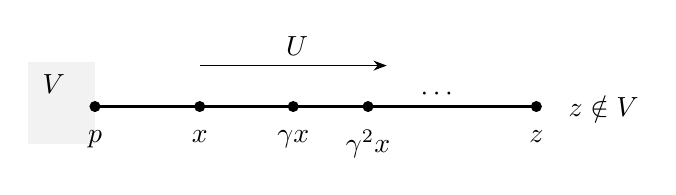
\begin{tikzpicture}[x=0.95cm,y=0.8cm,>=Stealth]
 \fill[gray!10] (-0.9,-0.6) rectangle (0,0.7);
 \node at (-0.55,0.35) {$V$};
 \draw[thick] (0,0)--(5.9,0);
 \fill (0,0) circle (2pt) node[below=5pt] {$p$};
 \fill (1.4,0) circle (2pt) node[below=5pt] {$x$};
 \fill (2.65,0) circle (2pt) node[below=5pt] {$\gamma x$};
 \fill (3.65,0) circle (2pt) node[below=5pt] {$\gamma^2x$};
 \node at (4.6,0.2) {$\cdots$};
 \fill (5.9,0) circle (2pt) node[below=5pt] {$z$};
 \draw[->] (1.4,0.65)--(3.9,0.65);
 \node[above] at (2.7,0.65) {$U$};
 \node[right] at (6.2,0) {$z\notin V$};
\end{tikzpicture}
\caption{The interval argument for an edge between higher-stage classes.
The element fixes the facing point $p$.  If it moves points of $U$
away from $p$, completeness supplies a second fixed endpoint $z$ outside
$V$.  The picture depicts betweenness in $\Phi$, not an arc in $B$.}
\label{fig:pretree-endpoint}
\end{figure}

Let $q\notin V$ be the second fixed point.  The points $p,q$ belong
to different $\sim_\beta$-classes; as $\beta\ge1$, their original
interval is infinite.  Lemma~\ref{pret:parabolic-star} makes $p$ terminal
in $\Phi$.  For every $v\in V$ and $u\in U$, formula~\eqref{pret:facing}
puts $p\in[u,v]$.  Since $p\ne u$, terminality forces $v=p$.
Thus $V=\{p\}$.  This vertex is a leaf of $\Sigma$: if it had two
neighbors, $p$ would lie strictly between representatives of them in
$\Phi$, again contradicting terminality.

Delete every edge with infinite stabilizer, together with its leaf
endpoint.  The remaining vertices form a nonempty invariant subtree.
Indeed, removing selected leaves preserves all paths between remaining
vertices.  If nothing remained, the original tree would have at most
two vertices.  Such an action without inversions has a fixed vertex,
which has already been excluded.  All remaining edges have finite
stabilizer, and a fixed vertex of the remaining tree would also be fixed
in $\Sigma$.

A finitely generated one-ended group acting without inversions on a
simplicial tree with finite edge stabilizers fixes a vertex
\cite[Lemma~6.6]{Bowditch1999Treelike}.  Applying this fact gives the
desired contradiction.

The least ordinal is therefore $\alpha=1$, which is exactly the
assertion of the lemma.
\end{proof}

\Needspace{14\baselineskip}
\subsection{The simplicial tree spanning the cut set}

The ordinal argument is complete.  We now work only with an ordinary
simplicial tree, whose vertices retain the separation information in $B$.

\begin{proposition}\label{pret:tree}
Let $\Gamma$ be a finitely presented torsion-free one-ended group with no
nontrivial splitting over a finite or two-ended subgroup.  Suppose it acts
minimally by convergence on a nondegenerate compact metric continuum $B$
whose set $P$ of global cut points is nonempty.  Then there is a
nontrivial minimal simplicial $\Gamma$-tree $\mathcal T$, with no edge
inversions and finite quotient, such that:
\begin{enumerate}[label=\textup{(\roman*)}]
\item $P$ is an invariant subset of its vertices, and every edge has one
endpoint in $P$ and one outside $P$;
\item $\mathcal T$ is spanned by $P$; its other vertices have degree at
least two;
\item every edge stabilizer is infinite;
\item if $a,b,q\in P$ and $q$ separates $a,b$ in $B$, then
$q\in[a,b]_{\mathcal T}$.
\end{enumerate}
Every point of $P$ is fixed by an infinite-order parabolic element.
\end{proposition}

\begin{proof}
Let $C\subset\Phi$ be the invariant finite-interval class supplied by
Lemma~\ref{pret:invariant-class}.  It contains more than one point,
because $\Phi$ has no fixed point.  Therefore its simplicial tree has
an edge, and Proposition~\ref{pret:package}\textup{(i)} places one
endpoint of that edge in $P$.

Choose $p\in C\cap P$.  The orbit $\Gamma p$ is dense in $B$ and lies
in $C$.  If $q\in P$, take an open separation of $B\setminus\{q\}$.
Both sides are nonempty open subsets of $B$, so each meets $\Gamma p$.
For orbit points $a,b$ on opposite sides, separation gives
$q\in[a,b]_{\Phi}$.  Since $C$ is full, $q\in C$.  We have proved
$P\subset C$.

Let $\mathcal T$ be the subtree of $C$ spanned by $P$, that is, the union
of the intervals between its points.  Its intervals agree with those of
$\Phi$, proving the asserted separation compatibility.  The adjacency
property gives the indicated bipartition and rules out edge inversions.
A vertex outside $P$ cannot be a leaf of a tree spanned by $P$.

To prove minimality, let $\mathcal S\subset\mathcal T$ be a nonempty
invariant subtree.  A singleton would be a fixed point of $\Phi$.
Otherwise $\mathcal S$ contains an edge, hence a point of $P$.
Its orbit is again dense in $B$; the separation argument of the preceding
paragraph gives $P\subset\mathcal S$.  Thus
$\mathcal S=\mathcal T$.

Choose a vertex $o$ and a finite generating set $S$ for $\Gamma$.
The union of the finitely many finite paths $[o,so]$, $s\in S$, is a
finite subtree after adjoining $o$.  Its translates form a connected
invariant subtree and therefore cover $\mathcal T$ by minimality.
Consequently the quotient has finitely many vertex and edge orbits.

Finally suppose an edge had finite stabilizer.  Collapsing the edges
outside its orbit gives a nontrivial tree with one edge orbit and a
minimal action without inversions.  Bass--Serre theory then yields a
nontrivial splitting over that edge stabilizer, contrary to the
hypotheses.  Thus every edge stabilizer is infinite.  The parabolic
assertion is Lemma~\ref{pret:parabolic-cuts}.
\end{proof}

\section{A continuum without cut points}\label{sec:blocks}

The remaining argument will use paths in a graph whose vertices accumulate
on a continuum without cut points.  We already have such a continuum if
the boundary $B$ has no cut points.  Otherwise, the cut-point tree provides
one of its blocks.  We construct the graph on that block and prove the
topological properties needed below.  In particular, none of the
arguments in this section assumes that $B$ is locally connected.

Recall that $X=\Gamma\sqcup B$ is our compact metric space, with metric
$\rho$, and that $B$ is a nondegenerate continuum.
Propositions~\ref{topo:dimension} and~\ref{topo:cech} give
\[
  \dim B\leq 1,
  \qquad
  \check H^1(B;\mathbb F_2)=0.
\]
Let $P$ be the set of cut points of $B$.  Throughout the construction
below, suppose that $P\ne\varnothing$.  By Proposition~\ref{pret:tree},
there is a nontrivial minimal simplicial $\Gamma$-tree $\mathcal T$
spanned by $P$, with finite quotient and bipartition into $P$ and the
remaining vertices.  All its edge stabilizers are infinite.  We will also
use its separation property: if $q\in P$ separates $a,b\in P$ in $B$,
then $q$ belongs to the open tree interval between $a$ and $b$.
Every point of $P$ is a parabolic fixed point.  In particular,
Lemma~\ref{dyn:parabolic} gives
\begin{equation}\label{block:parabolic-comparison}
  \rho(gp,g)\longrightarrow 0
  \quad\text{as }g\longrightarrow\infty\text{ in }\Gamma,
  \qquad p\in P.
\end{equation}
Here, and below, escape to infinity in a discrete group means escape
from every finite subset.

Choose a vertex $r\in\mathcal T\setminus P$, and write
\[
  R=\{p\in P: p\text{ is adjacent to }r\text{ in }\mathcal T\},
  \qquad H=\Gamma(r).
\]
Since $\mathcal T$ is spanned by $P$, a vertex outside $P$ cannot be a
leaf.  Thus $R$ has at least two points.  For distinct $a,b\in R$, their
tree interval is $a-r-b$.  The separation property therefore shows that
no cut point of $B$ separates $a$ and $b$.  Also, $H$ is exactly the
setwise stabilizer of $R$: an element preserving $R$ preserves the
unique midpoint $r$ of the interval between two distinct members of
$R$.

\subsection{A graph on the cut points}

The graph construction in Lemma~\ref{block:graph} adapts Bowditch's
peripheral-splitting construction~\cite[Section~4, Lemma~4.3 and its
proof]{Bowditch2001Peripheral}. We give the graph argument explicitly.
The subsequent near-path argument and continuous retraction are
extensions established here, not an invocation of a retraction theorem
from that source.

\begin{lemma}\label{block:graph}
There is a connected $\Gamma$-graph $K^*$ with vertex set $P$ and
finitely many edge orbits, such that the endpoints of each edge have
distance two in $\mathcal T$.  The graph $K$ induced by $K^*$ on $R$ is
connected and has finitely many $H$-orbits of vertices and edges.

Define $\pi:P\to R$ by letting $\pi(p)$ be the neighbor of $r$ on the
tree interval from $r$ to $p$.  An edge of $K^*$ with endpoints in $R$
is fixed by $\pi$, and every other edge is collapsed to a vertex.
Moreover, the stabilizer in $H$ of every vertex of $K$ is infinite.
\end{lemma}

\begin{proof}
The finite quotient of $\mathcal T$ gives finitely many $\Gamma$-orbits
in $P$.  Choose representatives $p_0,\ldots,p_k$ and a finite symmetric
generating set $S$ of $\Gamma$.  Start with the graph formed by all
translates of the edges from $p_0$ to $sp_0$, for $s\in S$, and from
$p_0$ to $p_i$, for $1\leq i\leq k$.  Omit loops.  The generator edges
connect the orbit of $p_0$, and the other edges connect every orbit to
it, so this graph is connected.  It has finitely many edge orbits.

Replace each edge by the consecutive pairs of $P$-vertices along the
tree interval between its endpoints.  These intervals are finite, and
the replacement is equivariant.  Thus the resulting graph $K^*$ is
still connected, still has finitely many edge orbits, and has the
required distance-two property.

For an edge $ab$ of $K^*$, let $a-s-b$ be its tree interval.  If $s=r$,
then $a,b\in R$ and $\pi$ fixes both endpoints.  If $s\ne r$, then
$a$ and $b$ lie in the same component of
$\mathcal T\setminus\{r\}$, so $\pi(a)=\pi(b)$.  This proves the
projection assertion.  Projecting a path between two members of $R$
and deleting stationary steps gives a path in $K$, proving its
connectedness.

If a group element carries one edge of $K$ to another, it carries their
unique tree midpoints to one another.  Both midpoints are $r$, so that
element lies in $H$.  Consequently, each $\Gamma$-orbit of edges in
$K^*$ meets $K$ in at most one $H$-orbit.  There are therefore finitely
many $H$-edge orbits in $K$.  Since $K$ is connected and has at least two
vertices, every vertex is incident to an edge; hence there are also
finitely many $H$-vertex orbits.  Finally, for $p\in R$, the stabilizer
$H_p$ is the stabilizer of the tree edge $rp$, which is infinite.
\end{proof}

The graph $K$ need not be locally finite, and its stabilizers need not
be finite.  These facts cause no difficulty: our arguments use finite
orbit sets, rather than finite valence or a proper graph action.

\begin{lemma}\label{block:near-path}
If $a_n,b_n\in P$ both tend to $x\in B$, there are paths in $K^*$ from
$a_n$ to $b_n$ all of whose vertices tend uniformly to $x$.

If the projections of the endpoints of a path in $K^*$ are distinct,
then, after stationary steps are removed, its projected path uses
only vertices of the original path.
\end{lemma}

\begin{proof}
Using the finitely many orbit representatives chosen in
Lemma~\ref{block:graph}, write
$a_n=g_np_{i_n}$ and $b_n=h_np_{j_n}$.  We may choose $g_n$ and $h_n$
to escape every finite subset of $\Gamma$: each representative has
infinite stabilizer, so there are infinitely many choices for each
representing element.  Equation~\eqref{block:parabolic-comparison},
applied to this finite list of representatives, gives
$g_n\to x$ and $h_n\to x$ in $X$.

By Lemma~\ref{compact:near-path}, there are Cayley graph paths from
$g_n$ to $h_n$ whose vertices tend uniformly to $x$.  Fix finite
$K^*$-paths from $p_0$ to $sp_0$ for each Cayley generator $s$, and
from $p_0$ to each representative $p_i$.  Replace a Cayley step
$g\longrightarrow gs$ by the $g$-translate of the first appropriate
path.  At the endpoints, use the translates of the paths to $p_{i_n}$
and $p_{j_n}$.  The result is a $K^*$-path from $a_n$ to $b_n$.

Only finitely many points $t\in P$ occur in the fixed path templates.
For each such point, $\rho(gt,g)\to0$ as $g$ escapes, by
\eqref{block:parabolic-comparison}.  The Cayley path vertices escape
finite sets uniformly, because they tend uniformly to the boundary
point $x$.  Hence all vertices of the transferred paths tend uniformly
to $x$ as well.

For the last assertion, Lemma~\ref{block:graph} says that every
nonconstant projected edge was already an edge of the original path.
When the projected endpoints differ, every vertex of the projected
path after stationary steps are removed is incident to one of these
edges.  It therefore occurred in the original path.
\end{proof}

\subsection{Retraction onto a block}

\begin{proposition}\label{block:retraction}
The map $\pi:P\to R$ extends to a continuous retraction
\[
  \mathfrak r:B\longrightarrow L,
  \qquad L=\overline R^{\,B},
\]
which is locally constant on $B\setminus L$.  The space $L$ is a
nondegenerate continuum without cut points, and
\[
  \dim L\leq1,
  \qquad \check H^1(L;\mathbb F_2)=0.
\]
\end{proposition}

\begin{proof}
By the minimality established in Proposition~\ref{dyn:minimal}, the
nonempty invariant set $P$ is dense in $B$.  We first determine the
limit of $\pi(p_n)$ whenever $p_n\in P$ tends to a point of $B$.

Let $x\in B\setminus L$, and choose a neighborhood $O$ of $x$ in $B$
disjoint from $L$.  The map $\pi$ is constant on $P\cap V$ for some
neighborhood $V\subset O$ of $x$.  Otherwise, we could choose
$a_n,b_n\to x$ with $\pi(a_n)\ne\pi(b_n)$.
Lemma~\ref{block:near-path} would join them by paths whose vertices
eventually all lie in $O$.  Their nonconstant projected paths contain
vertices in $R$ that also belong to the original paths.  This
contradicts $O\cap R=\varnothing$.

Now let $x\in L$ and $a_n\in P$ tend to $x$.  Choose $b_n\in R$ tending
to $x$, and join $a_n$ to $b_n$ by the paths supplied by
Lemma~\ref{block:near-path}.  Whenever $\pi(a_n)\ne b_n$, the same
Lemma places $\pi(a_n)$ on the original path.  Therefore
$\pi(a_n)\to x$.  The indices for which $\pi(a_n)=b_n$ satisfy the
same conclusion directly.

Take the closure of the graph of $\pi$ in $B\times L$.  Density of
$P$ and compactness of $L$ show that this closed set projects onto
$B$.  The preceding two paragraphs show that it has exactly one point
over each point of $B$.  Its projection onto $B$ is consequently a
continuous bijection from a compact space to a Hausdorff space, hence
a homeomorphism.  The second coordinate defines the desired
continuous map $\mathfrak r$.  It is the identity on $L$, and the
first paragraph makes it locally constant on $B\setminus L$.

Since $B$ is connected, its image $L$ is connected.  The set $R$ has at
least two points, so $L$ is nondegenerate.  The dimension bound follows
because $L$ is a closed subset of the compact metric space $B$.
If $i:L\hookrightarrow B$ denotes inclusion, then
$\mathfrak r\circ i=\operatorname{id}_L$.  Functoriality of \v Cech
cohomology gives
$i^*\mathfrak r^*=\operatorname{id}_{\check H^1(L;\mathbb F_2)}$.
Thus $\mathfrak r^*$ injects this group into
$\check H^1(B;\mathbb F_2)=0$.

It remains to rule out a cut point of $L$.  Suppose that
$L\setminus\{q\}=U\sqcup V$ is a separation into nonempty open sets.
Density supplies $a\in R\cap U$ and $b\in R\cap V$.  The extra fiber
\[
  F=\mathfrak r^{-1}(\{q\})\setminus\{q\}
\]
is closed in $B\setminus\{q\}$ by continuity.  It is also open there:
it lies in $B\setminus L$, where $\mathfrak r$ is locally constant.
Consequently,
\[
 B\setminus\{q\}
   =\bigl(\mathfrak r^{-1}(U)\cup F\bigr)
      \sqcup\mathfrak r^{-1}(V)
\]
is a separation, with $a$ and $b$ on opposite sides.  This would make
$q$ a cut point of $B$ separating two members of $R$, contrary to the
separation property of the tree noted above.  Hence $L$ has no cut
points.
\end{proof}

\subsection{The common setting for path pushing}

We now include the case $P=\varnothing$ and collect the exact inputs
for path pushing. The first two properties below retain the boundary
topology and convergence dynamics. The graph conditions describe how
vertices and edges approach the boundary: finite orbit sets and comparison
with group vertices will control edge lengths even when the graph has
infinite valence. When graph vertices lie in the boundary, stabilizer
powers send any prescribed finite set of boundary points toward the
vertex they fix; this will connect
the convergence dynamics to graph components during path pushing.
All closures and metrics in the following proposition are inherited
from $X$.

\begin{proposition}\label{block:setting}
There are a subgroup $H\leq\Gamma$, a compact space
$Y=H\sqcup L\subset X$, and a connected $H$-graph $K$ with vertex set
$I\subset Y$, with the following properties.
\begin{enumerate}
\item $Y=\overline H^{\,X}$.  The points of $H$ are isolated in $Y$,
and $L$ is a nondegenerate continuum without cut points satisfying
\[
  \dim L\leq1,
  \qquad \check H^1(L;\mathbb F_2)=0.
\]
\item If $h_n\to a\in L$ and $h_n^{-1}\to b\in L$, then $h_n$
converges to the constant map $a$, uniformly on compact subsets of
$Y\setminus\{b\}$.
\item The graph $K$ has finitely many $H$-orbits of vertices and
edges.  Either $I=H$, or $I\subset L$.  Every point of $L$ is the limit
of a sequence of distinct vertices in $I$.
\item For each fixed $w\in I$,
\begin{equation}\label{block:comparison}
  \rho(hw,h)\longrightarrow0
  \quad\text{as }h\longrightarrow\infty\text{ in }H.
\end{equation}
\item For every $x\in L$ and every neighborhood $W$ of $x$ in $Y$,
there is a neighborhood $V$ of $x$ in $Y$ such that any two vertices
of $I\cap V$ can be joined by a path in $K$ all of whose vertices
belong to $W$.
\item If $I\subset L$, then for each $p\in I$ there is an
infinite-order element $h\in H_p$ such that
\[
  h^jz\longrightarrow p
  \quad(j\longrightarrow+\infty),\qquad z\in L.
\]
\end{enumerate}
No finite generation assumption on $H$ or local finiteness assumption
on $K$ is included in these conclusions.
\end{proposition}

\begin{proof}
If $P=\varnothing$, take $H=\Gamma$, $Y=X$, $L=B$, and let $K$ be the
original Cayley graph, with $I=H$.  The continuum properties are those
already proved for $B$, and absence of cut points is the definition of
this case.  The closure, convergence, finite orbit, and near-path
assertions follow from the construction of $X$,
Proposition~\ref{dyn:convergence}, and
Lemma~\ref{compact:near-path}.  Every boundary point is approached by
distinct group vertices, since the group vertices are isolated and
dense in $X$.

For completeness, the comparison assertion in this case also follows
from convergence.  If it failed for a fixed $w\in H$, choose escaping
$h_n$ with $\rho(h_nw,h_n)$ bounded away from zero.  After passing to a
subsequence, compactness gives $h_n\to a\in B$ and
$h_n^{-1}\to b\in B$.  Since $w\in H$ is different from $b$,
Proposition~\ref{dyn:convergence} gives $h_nw\to a$, a contradiction.
The last assertion has no content in this case.

If $P\ne\varnothing$, use the objects constructed above:
\[
  H=\Gamma(r),\qquad I=R,\qquad
  L=\overline R^{\,B},\qquad Y=H\sqcup L,
\]
and let $K$ be the graph of Lemma~\ref{block:graph}.
The continuum and finite orbit assertions follow from that Lemma and
Proposition~\ref{block:retraction}.  We verify the remaining
interfaces explicitly.

First, $Y=\overline H^{\,X}$.  Fix $p\in R$.  If an escaping sequence
$h_n\in H$ converges to a boundary point, then
\eqref{block:parabolic-comparison} and $h_np\in R$ show that its limit
belongs to $L$.  Conversely, for any $p\in R$, the infinite stabilizer
$H_p$ supplies distinct elements $h_n$ with $h_np=p$.
Equation~\eqref{block:parabolic-comparison} gives $h_n\to p$.  Thus
$R\subset\overline H^{\,X}$, and taking closures gives
$L\subset\overline H^{\,X}$.  No point of $\Gamma\setminus H$ belongs
to this closure, since all group vertices are isolated.  This proves
the equality and compactness of $Y$.  The subgroup $H$ preserves both
$L$ and $Y$, and the convergence assertion is the restriction of
Proposition~\ref{dyn:convergence}.

The set $R$ is dense in the nondegenerate continuum $L$, which has no
isolated points.  It follows that every point of $L$ is approached by
distinct members of $R$: otherwise a sufficiently small neighborhood
would meet $R$ in at most one point and make that point isolated in
$L$.  Equation~\eqref{block:comparison} is exactly
\eqref{block:parabolic-comparison} restricted to $H$.

For the near-path assertion, take two sequences in $R$ tending to the
same point of $L$.  Lemma~\ref{block:near-path} joins them by $K^*$-paths
whose vertices tend uniformly to that point.  Project to $R$.  If the
endpoints differ, the projected paths use only vertices of the
original paths; if they agree, use the constant path.  Thus the
projected $K$-paths still tend uniformly to that point.  In metric
spaces this sequential statement gives the stated neighborhood
formulation: a failure for some $W$ would yield endpoints in
successively smaller balls that cannot be joined inside $W$.

Finally, $H_p$ is infinite by Lemma~\ref{block:graph}.  Since $\Gamma$
is torsion-free, it contains an infinite-order element.  The
cut-point stabilizer conclusions in Lemma~\ref{pret:parabolic-cuts}
make this element parabolic with fixed point $p$.  Its powers have
the asserted dynamics by Lemma~\ref{dyn:parabolic}.
\end{proof}

\section{Component labels and annular depth}
\label{sec:annuli}

The graph paths supplied by Proposition~\ref{block:setting} stay near a
boundary point, but they may pass through vertices that we need to remove.
We first show how to assign a component of the remaining graph to a nearby
boundary point. We then construct an invariant integer-valued depth on
group vertices. These are the two inputs for pushing paths towards the
boundary in the next section.

We use the following setting from Proposition~\ref{block:setting}.
The compact metric space $(Y,\rho)$ is the disjoint union $H\sqcup L$,
where $H$ is a group, its points are isolated, and $H$ acts on $Y$ by
homeomorphisms extending left multiplication. The space $L$ is a
nondegenerate continuum, has no cut point, and satisfies
$\dim L\leq 1$ and $\check H^1(L;\mathbb F_2)=0$.
If distinct elements $g_n\in H$ satisfy $g_n\to a$ and
$g_n^{-1}\to b$, then $a,b\in L$ and $g_n$ converges to $a$ uniformly
on compact subsets of $Y\setminus\{b\}$.

There is a connected $H$-graph $K$ with vertex set $I$, where either
$I=H$ or $I\subset L$. It has finitely many vertex and edge orbits.
Every point of $L$ is a limit of distinct vertices of $K$, and, for every
$x\in L$ and neighborhood $W$ of $x$ in $Y$, there is a neighborhood
$V$ of $x$ such that any two vertices in $I\cap V$ can be joined by a
finite path of $K$ whose vertices lie in $W$.
For each fixed $w\in I$,
\[
  \rho(gw,g)\longrightarrow 0
  \qquad(g\in H\text{ leaving every finite set}).
\]
When $I\subset L$, every $p\in I$ has an infinite-order stabilizer
element $h\in H$ for which $h^jz\to p$ for every $z\in L$ as
$j\to+\infty$. No local finiteness of $K$ or finite generation of $H$
is assumed here.

\subsection{Extending labels across a deleted point}

We write $k=\mathbb F_2$ with its discrete topology. A locally constant
map to $k$ records a division into two open and closed parts.
The cohomology hypothesis prevents such a division from appearing only
after one point has been removed from a small neighborhood.
The circle shows why absence of cut points alone would not suffice:
removing the midpoint of a small open arc leaves two sides that can
carry different constant labels.

\begin{lemma}\label{ann:extension}
Let $L$ be a nondegenerate compact metric continuum with no cut point and
$\check H^1(L;k)=0$. If $x\in L$ and $V$ is an open neighborhood of $x$
in $L$, every locally constant map $u:V\setminus\{x\}\to k$ extends
uniquely to a locally constant map on $V$.
\end{lemma}

\begin{proof}
Put $U=L\setminus\{x\}$. We prove directly, using finite-cover
cohomology, that there are locally constant maps $f_U:U\to k$ and
$f_V:V\to k$ such that
\[
  u=f_U+f_V\quad\text{on }U\cap V.
\]
Choose open sets $U_0,V_0$ covering $L$ whose closures are contained in
$U,V$, respectively. The set
$C=\overline{U_0}\cap\overline{V_0}$ is a compact subset of $U\cap V$.
Its two subsets $C\cap u^{-1}(0)$ and $C\cap u^{-1}(1)$ are disjoint
compact sets. Choose $\delta>0$ smaller than their distance when both
are nonempty; if either is empty, any positive $\delta$ suffices.

Take a finite open cover $(W_i)$ of $L$ refining $(U_0,V_0)$, with each
$W_i$ of diameter less than $\delta$, and give it a parent
$P_i\in\{U,V\}$ according to this refinement. On every nonempty
$W_i\cap W_j$, define $c_{ij}=0$ if $P_i=P_j$, and define $c_{ij}$ to
be the value of $u$ there otherwise. This latter value is constant:
the intersection lies in $C$ and cannot meet both of its two compact
parts. At a triple intersection either all parents agree, or exactly
two of the three transition values equal the same value of $u$.
Thus $(c_{ij})$ is a $1$-cocycle on the nerve of $(W_i)$.

Since $\check H^1(L;k)=0$, some finite open refinement $(Z_\alpha)$,
with refinement map $r$, admits constants $a_\alpha\in k$ satisfying
\[
  a_\alpha+a_\beta=c_{r(\alpha)r(\beta)}
  \quad\text{whenever }Z_\alpha\cap Z_\beta\ne\varnothing.
\]
For $z\in U\cap Z_\alpha$, set $f_U(z)=a_\alpha$ if
$P_{r(\alpha)}=U$, and set $f_U(z)=a_\alpha+u(z)$ otherwise.
The displayed identity makes these definitions agree on overlaps.
They are locally constant. Define $f_V$ by the same rule, with $U,V$
interchanged. Then $f_U+f_V=u$ on $U\cap V$.

Since $x$ is not a cut point, $U$ is connected, so $f_U$ has one
constant value, say $c$. The map $f_V+c$ is the required extension.
Uniqueness follows because a nondegenerate continuum has no isolated
points, so $V\setminus\{x\}$ is dense in $V$.
\end{proof}

For a set $D\subset Y$, denote by $D'$ the set of limits in $Y$ of
sequences of distinct points of $D$. In a metric space $D'$ is closed.
For an allowed vertex set $T\subset I$, put
\[
  \Omega_T=L\setminus(I\setminus T)'.
\]
This is precisely the open set of boundary points near which deleted
vertices do not accumulate as distinct points. We use graph components
of the induced graph $K[T]$.

\begin{lemma}\label{ann:component}
In the setting above, each $x\in\Omega_T$ determines a unique component
$Q_T(x)$ of $K[T]$ such that all allowed vertices in some neighborhood
of $x$ belong to $Q_T(x)$. Every $x\in\Omega_T$ is a limit of distinct
allowed vertices, and the assignment $Q_T$ is locally constant on
$\Omega_T$. If $t\in T\cap L\cap\Omega_T$, then $Q_T(t)$ is the
component containing the vertex $t$ itself.
\end{lemma}

\begin{proof}
There is a neighborhood $W$ of $x$ such that
$(I\setminus T)\cap W\subset\{x\}$. Since $x$ is a limit of distinct
vertices of $I$, it is consequently a limit of distinct vertices of
$T$ as well.

Suppose first that $x$ is not a deleted vertex. After shrinking $W$,
it contains no deleted vertex. The near-path property then puts all
vertices sufficiently near $x$ in one component of $K[T]$. There are
allowed vertices arbitrarily near $x$, so this component is unique.
The same neighborhood, together with approximation by allowed vertices,
shows that the component assignment is locally constant near $x$.
When $x$ itself is an allowed vertex, it belongs to this component.

The remaining case has $I\subset L$ and $x\in I\setminus T$.
Choose an open neighborhood $V$ of $x$ in $L$ containing no other
deleted vertex. By the preceding case, every $y\in V\setminus\{x\}$
has a component label, and these labels form a locally constant map
\[
  q:V\setminus\{x\}\longrightarrow\{\text{components of }K[T]\}.
\]
Every map from this label set to $k$, composed with $q$, extends across
$x$ by Lemma~\ref{ann:extension}. We claim this forces $q$ itself to
be constant sufficiently near $x$.

To see this, call a label recurrent if it occurs arbitrarily near $x$.
If two labels are recurrent, a coloring separating them contradicts
the extension property. If exactly one label is recurrent but $q$ is
not eventually constant, color that label $0$ and all others $1$ to
obtain the same contradiction. If no label is recurrent, a sequence
of points tending to $x$ can be chosen with pairwise distinct labels:
at each step, first exclude the finitely many labels already chosen.
Color these successive labels alternately $0$ and $1$.
This again contradicts extension as a locally constant map.
Thus one component label occurs throughout a small punctured
neighborhood of $x$. Every allowed vertex there belongs to its own
label by the first case, so all these vertices belong to that component.

This proves existence at a deleted vertex too. Approximation by allowed
vertices proves uniqueness and, on shrinking the neighborhood once
more, local constancy of $Q_T$ there.
\end{proof}

\subsection{An invariant system of annuli}

We use the annulus-system method of
\cite[Sections~6--7]{Bowditch1998Topological}, with the following
nesting convention. The construction and the two properties needed
here are proved explicitly; the sides need not be connected.

An \emph{annulus} in $Y$ is an ordered pair
$\sigma=(\sigma^-,\sigma^+)$ of disjoint closed subsets of $Y$ such
that each side meets $L$ and $\sigma^-\cup\sigma^+\ne Y$. Its sides
need not be connected. For annuli $\sigma,\tau$, write
\[
  \sigma<\tau\quad\Longleftrightarrow\quad
  \sigma^+\cup\tau^-=Y.
\]
Then $\sigma^-\subset\operatorname{int}(\tau^-)$ and
$\tau^+\subset\operatorname{int}(\sigma^+)$. The relation is transitive
and irreflexive. Thus a nested chain
$\sigma_1<\cdots<\sigma_n$ contains distinct annuli.
A chain goes \emph{from $F$ to $E$} if
$F\subset\sigma_1^-$ and $E\subset\sigma_n^+$.

\begin{lemma}\label{ann:system}
There is a set $\mathcal A$ of annuli invariant under $H$ and under
interchange of the two sides, with the following properties.
\begin{enumerate}
\item For every $\delta>0$, only finitely many annuli in $\mathcal A$
have both sides of diameter at least $\delta$.
\item For every closed $F\subset Y$, every $x\in L\setminus F$, and
every integer $n\geq1$, there is a chain of $n$ annuli in $\mathcal A$
from $F$ to a neighborhood of $x$ in $Y$.
\end{enumerate}
\end{lemma}

\begin{proof}
We first record a uniform consequence of convergence. For every
$r,\varepsilon>0$, all but finitely many $g\in H$ admit a point
$b_g\in L$ such that
\[
  \operatorname{diam}g\bigl(Y\setminus B_\rho(b_g,r)\bigr)
  <\varepsilon.
\]
Otherwise choose distinct exceptions $g_n$ and pass to a subsequence
with $g_n\to a\in L$ and $g_n^{-1}\to b\in L$. Uniform convergence
on the compact set $Y\setminus B_\rho(b,r)$ gives a contradiction.

Choose $r_i\downarrow0$ with $r_i<\operatorname{diam}(L)/3$, and put
$\varepsilon_i=2^{-i}$. Apply the preceding observation with
$r=r_i/4$ and $\varepsilon=\varepsilon_i$, obtaining a finite
exceptional set $E_i\subset H$. Uniform continuity of the finitely
many maps in $E_i$ permits a common choice $0<s_i<r_i/4$ such that
\[
  \operatorname{diam}g\bigl(\overline{B_\rho(y,s_i)}\bigr)
  <\varepsilon_i
  \quad(g\in E_i,\ y\in L).
\]
Choose finitely many centers $y_{ij}\in L$ whose $s_i/2$-balls cover
$L$. At each center take the seed annulus
\[
  \sigma_{ij}^- =Y\setminus B_\rho(y_{ij},r_i),
  \qquad
  \sigma_{ij}^+ =\overline{B_\rho(y_{ij},s_i)}.
\]
Its sides are disjoint and have distance at least $r_i-s_i$.
The positive side contains its center. The negative side meets $L$
because every point of $L$ is at distance at least
$\operatorname{diam}(L)/2$ from some point of $L$.
The sides cannot cover $L$, since their nonempty closed intersections
with $L$ would disconnect it.

Let $\mathcal A$ consist of all distinct translates of these annuli
and their reversals. A ball of radius $r_i/4$ cannot meet both sides
of a seed annulus, whose mutual distance exceeds $3r_i/4$.
For $g\notin E_i$, one side therefore lies outside the exceptional
ball for $g$ and has image of diameter less than $\varepsilon_i$.
For $g\in E_i$, the positive side has that property by the choice of
$s_i$. Consequently every translated level-$i$ annulus has at least
one side of diameter less than $\varepsilon_i$.

For a fixed seed and fixed $\delta>0$, only finitely many distinct
translates can have both sides of diameter at least $\delta$.
If not, choose corresponding distinct group elements and a convergence
subsequence with repeller $b$. At least one of the two closed seed
sides excludes $b$, so its images have diameter tending to zero.
There are only finitely many seeds at each level, and levels with
$\varepsilon_i<\delta$ contribute no annuli with two such large sides.
This proves the first assertion.

For the second assertion, let $F$ be closed and $x\in L\setminus F$.
At a sufficiently fine level, choose a center $y_{ij}$ with
$\rho(x,y_{ij})<s_i/2$ and
$r_i+s_i/2<\operatorname{dist}(x,F)$ when $F$ is nonempty.
The negative side contains $F$, and the positive side contains a
neighborhood of $x$. Suppose an annulus already chosen has positive
side containing $B_\rho(x,\eta)$. Choose a finer level with
$r_j+s_j/2<\eta$, and a center $y$ within $s_j/2$ of $x$.
Then $B_\rho(y,r_j)\subset B_\rho(x,\eta)$, so the new annulus is
larger in the order $<$, and its positive side again contains a
neighborhood of $x$. Repeating gives any prescribed finite length.
\end{proof}

Fix such a system $\mathcal A$. For $F\subset Y$ and $v\in Y$, define
\[
  D(F,v)=\sup\{n\geq1:
       \text{a chain of length }n\text{ in }\mathcal A
       \text{ goes from }F\text{ to }\{v\}\},
\]
with value $0$ if there is no such chain. In general the value belongs
to $\{0,1,2,\ldots\}\cup\{\infty\}$. We abbreviate $D(\{u\},v)$
to $D(u,v)$. This function counts separating annuli; it is not asserted
to be a metric.

\begin{lemma}\label{ann:depth}
For $g\in H$, $F\subset Y$, and $v\in Y$,
\[
  D(gF,gv)=D(F,v).
\]
If $F$ contains a point of $H$ and $v\in H$, then $D(F,v)$ is finite.
When it is positive, a chain attains this finite maximum.
If $F$ is closed, $x\in L\setminus F$, and $N\geq1$, there is a
neighborhood $V_N$ of $x$ in $Y$ such that $D(F,v)\geq N$ for every
$v\in V_N$.
\end{lemma}

\begin{proof}
Translation carries annuli and chains bijectively to annuli and chains,
which proves equivariance. Suppose $h\in F\cap H$ and $v\in H$.
As $L$ is closed and excludes $h,v$, the number
\[
  \delta=\min\{\operatorname{dist}(h,L),
                    \operatorname{dist}(v,L)\}
\]
is positive. Throughout a chain from $F$ to $v$, every negative side
contains $h$ and meets $L$, and every positive side contains $v$ and
meets $L$. Both sides therefore have diameter at least $\delta$.
Lemma~\ref{ann:system} supplies only finitely many such annuli, and a
strict chain cannot repeat one. This proves finiteness. A finite
nonzero supremum of possible integer lengths is attained.
The final assertion is precisely the second part of
Lemma~\ref{ann:system}, using its terminal neighborhood.
\end{proof}

\section{Pushing paths and local connectedness}\label{sec:path-pushing}

We work in the setting of Proposition~\ref{block:setting}, with compact
metric space $Y=H\sqcup L$ and graph $K$ on $I$, and use the annulus system
of Lemma~\ref{ann:system}.  Our aim is to turn paths near a point of $L$
into connected subsets of $L$.  To do this we push the paths arbitrarily
far from a fixed closed set and then take limits of their vertex sets.
The graph can have infinite valence and infinite vertex stabilizers;
none of the arguments below requires finite generation of $H$.

At a fixed depth, nearby boundary points determine components of the
remaining graph. We will prove that, beyond one common threshold,
increasing the depth cannot separate points with the same component
label. Iterating this fact produces a single boundary neighborhood whose
points retain the same component label at every greater depth. Limits
of the resulting graph paths will then lie entirely in the boundary.

\subsection{A uniform depth comparison}

Fix a closed subset $A\subset Y$ with $1\in A$ and $L\setminus A\ne\varnothing$.
The annular depth $D(F,v)$ is the maximum length of a chain from $F$ to $v$
when it is finite, as in Lemma~\ref{ann:depth}.  Write
\[
 d_0=\operatorname{dist}(1,L)>0,
 \qquad
 N(a,b)=\#\{\sigma:
       \operatorname{diam}\sigma^-\ge a,
       \operatorname{diam}\sigma^+\ge b\}\quad(a,b>0).
\]
The number $N(a,b)$ is finite by Lemma~\ref{ann:system}.  A side containing
$1$ has diameter at least $d_0$, because every side meets $L$.

\begin{lemma}\label{push:shrinking}
Let $g_n\in H$ satisfy $D(A,g_n)\to\infty$, and set $F_n=g_n^{-1}A$.
After passage to a subsequence there is $q\in L$ such that $F_n$ converges
in the Hausdorff metric to $\{q\}$.
\end{lemma}
\begin{proof}
By equivariance, $D(F_n,1)=D(A,g_n)$.  In any chain from $F_n$ to $1$,
every positive side contains $1$.  If the chain has more than
$N(\epsilon,d_0)$ members, one of its negative sides has diameter less
than $\epsilon$.  This side contains $F_n$.  Hence
$\operatorname{diam}F_n\to0$.

Lemma~\ref{ann:depth} gives $D(A,g)<\infty$ for each fixed $g\in H$.
Thus $g_n$ escapes every finite subset of $H$, as does $g_n^{-1}$.
Since $1\in A$, we have $g_n^{-1}\in F_n$.  Compactness of $Y$ and
isolatedness of its group vertices give a subsequence
$g_n^{-1}\to q\in L$.  The diameter conclusion now gives the assertion.
\end{proof}

\begin{lemma}\label{push:depth-comparison}
Suppose $F_n=g_n^{-1}A$ converges to $\{q\}$ as in
Lemma~\ref{push:shrinking}.  For each $r>0$, set
\[
 C_r=N(r/2,d_0)+N(d_0,r)+2.
\]
For all sufficiently large $n$, uniformly over every $b\in H$ with
$\rho(b,q)\ge3r$, one has
\begin{equation}\label{eq:push-depth-comparison}
 D(F_n,b)\ge D(F_n,1)+D(\{1\},b)-C_r.
\end{equation}
Consequently, if $b_n\in H$ tends to $z\in L\setminus\{q\}$, then
\[
 D(F_n,b_n)\ge D(F_n,1)+D(\{1\},b_n)-C
 \quad\hbox{and}\quad D(\{1\},b_n)\longrightarrow\infty
\]
for a constant $C$ independent of $n$.
\end{lemma}
\begin{proof}
Choose $n$ large enough that
$F_n\subset B(q,r/2)$ and
$\ell=D(F_n,1)>N(r/2,d_0)+1$.  Take a chain
$\sigma_1<\cdots<\sigma_\ell$ of maximum length from $F_n$ to $1$,
and put $U=B(q,r)$.
If $\sigma_j^-\not\subset U$, its negative side contains a point of
$F_n$ and a point outside $U$, so has diameter at least $r/2$.
Its positive side has diameter at least $d_0$.
There are therefore at most $N_-=N(r/2,d_0)$ such annuli.
Because negative sides increase along a chain, these form a terminal
segment.  Remove that segment and one further annulus.
The retained initial chain has at least $\ell-N_--1$ members.
The negative side of the next annulus lies in $U$, so the last retained
positive side contains $Y\setminus U$.
In particular, this retained chain already ends on the side containing
any $b$ under consideration.

Let $t=D(\{1\},b)$, and take a maximum chain
$\tau_1<\cdots<\tau_t$ from $1$ to $b$ when $t>0$.
Put $V=Y\setminus\overline{B(q,2r)}$.
A positive side not contained in $V$ contains both $b$ and a point at
distance at most $2r$ from $q$, so has diameter at least $r$.
Every negative side contains $1$, so has diameter at least $d_0$.
Thus at most $N_+=N(d_0,r)$ positive sides fail to lie in $V$;
these form an initial segment.
If $t>N_++1$, remove this initial segment and one further annulus.
The retained final chain has at least $t-N_+-1$ members, and its first
negative side contains $Y\setminus V$.

Since $U\cap V=\varnothing$, the last positive side of the first retained
chain and the first negative side of the second cover $Y$.
The defining order relation therefore concatenates the two chains.
Their total length is at least $\ell+t-N_--N_+-2$.
If $t\le N_++1$, the first retained chain alone has at least this length.
This proves \eqref{eq:push-depth-comparison}, including a constant and
threshold independent of $b$.

For the final assertion choose $r$ with $4r<\rho(q,z)$.
Eventually $\rho(b_n,q)\ge3r$, so the inequality applies.
For any prescribed integer $N$, Lemma~\ref{ann:system} supplies a chain
of length $N$ from $\{1\}$ to a neighborhood of $z$.
Eventually this neighborhood contains $b_n$, proving
$D(\{1\},b_n)\to\infty$.
\end{proof}

Figure~\ref{fig:annular-chains} illustrates this pruning and
concatenation for a sequence $b_n\to z\ne q$.
\begin{figure}[!htbp]
\centering
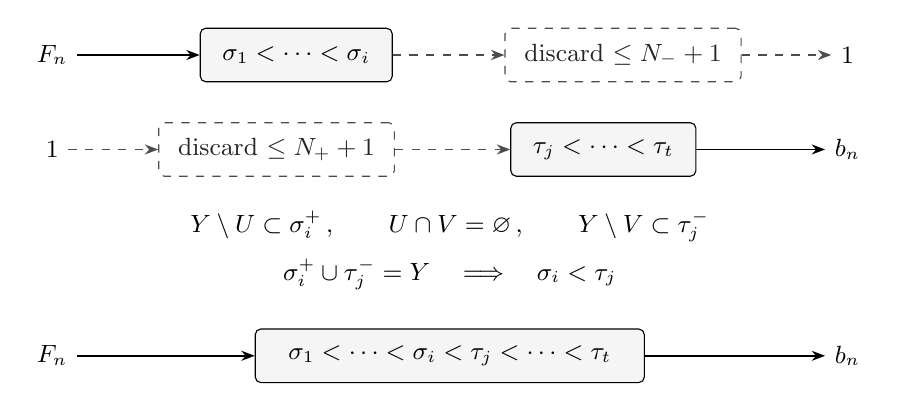
\begin{tikzpicture}[
  x=1cm,y=1cm,
  every node/.style={font=\small},
  retained/.style={draw,rounded corners=2pt,fill=black!4,
    minimum height=0.68cm,inner xsep=8pt},
  omitted/.style={draw=black!70,dashed,rounded corners=2pt,
    text=black!85,minimum height=0.68cm,inner xsep=7pt},
  link/.style={-{Stealth[length=1.7mm]},semithick},
  discarded/.style={link,dashed,draw=black!70}
]
\node (f) at (0,0) {$F_n$};
\node[retained] (sig) at (3.1,0)
  {$\sigma_1<\cdots<\sigma_i$};
\node[omitted] (tail) at (7.25,0) {discard $\le N_-+1$};
\node (onea) at (10.1,0) {$1$};
\draw[link] (f) -- (sig);
\draw[discarded] (sig) -- (tail);
\draw[discarded] (tail) -- (onea);

\node (oneb) at (0,-1.2) {$1$};
\node[omitted] (head) at (2.85,-1.2) {discard $\le N_++1$};
\node[retained] (tau) at (7,-1.2)
  {$\tau_j<\cdots<\tau_t$};
\node (b) at (10.1,-1.2) {$b_n$};
\draw[discarded] (oneb) -- (head);
\draw[discarded] (head) -- (tau);
\draw[link] (tau) -- (b);

\node[align=center] at (5.05,-2.48) {
  $Y\setminus U\subset\sigma_i^+\,,\qquad
   U\cap V=\varnothing\,,\qquad
   Y\setminus V\subset\tau_j^-$\\[5pt]
  $\sigma_i^+\cup\tau_j^-=Y\quad\Longrightarrow\quad
   \sigma_i<\tau_j$
};
\node[retained,inner xsep=12pt] (joined) at (5.05,-3.82)
  {$\sigma_1<\cdots<\sigma_i<\tau_j<\cdots<\tau_t$};
\node (fj) at (0,-3.82) {$F_n$};
\node (bj) at (10.1,-3.82) {$b_n$};
\draw[link] (fj) -- (joined);
\draw[link] (joined) -- (bj);
\end{tikzpicture}
\caption{Concatenating annular chains after bounded pruning. Choose
fixed disjoint neighborhoods $U$ of $q$ and $V$ of $z$, where
$F_n$ shrinks to $q$ and $b_n\to z\ne q$.
The terminal positive side of the first retained chain contains
$Y\setminus U$; the initial negative side of the second contains
$Y\setminus V$. Their union is $Y$, which is exactly the annulus-order
criterion for joining the chains. The diagram records order and
containment only; the sides need not be connected.}
\label{fig:annular-chains}
\end{figure}


\subsection{Components of the deeper vertex sets}

Choose one representative $p_i$ for each of the finitely many
$H$-orbits in $I$.  When $I=H$, use only $p_1=1$.
For a vertex $u$ in the orbit of $p_i$, define its set of representatives
in the group by
\[
 C(u)=\{g\in H:g p_i=u\}.
\]
For integers $m\ge0$ define
\begin{equation}\label{eq:push-deep-vertices}
 I_m=\left\{u\in I\setminus A:
           \min_{g\in C(u)}D(A,g)\ge m\right\}.
\end{equation}
Each depth in this minimum is a finite nonnegative integer, so the
minimum exists.  The condition concerns \emph{every} representative of
$u$.  This will allow us to move through an infinite stabilizer without
losing the depth bound.

\begin{lemma}\label{push:component-labels}
For each fixed $m$, the deleted vertices $I\setminus I_m$ have no
accumulation by distinct vertices at any point of $L\setminus A$.
Consequently Lemma~\ref{ann:component} defines a locally constant map
\[
 Q_m:L\setminus A\longrightarrow
      \{\text{components of }K[I_m]\},
\]
whose value at $x$ contains all vertices of $I_m$ sufficiently near $x$.
Every $x\in L\setminus A$ is approached by distinct vertices with this
label.  Moreover, for each finite subset $E\subset I$ one has
$E\cap I_m=\varnothing$ for all sufficiently large $m$.
\end{lemma}
\begin{proof}
For $m=0$ the first assertion follows from $I_0=I\setminus A$.
Suppose $m\ge1$.
Suppose that distinct $u_n\in I\setminus I_m$ tend to
$x\in L\setminus A$.
Eventually $u_n\notin A$, so choose $a_n\in C(u_n)$ with $D(A,a_n)<m$.
Since there are only finitely many orbit representatives and the $u_n$
are distinct, $a_n$ escapes every finite subset of $H$.
The comparison $\rho(gp_i,g)\to0$ in Proposition~\ref{block:setting},
applied to the finite list of representatives, gives $a_n\to x$.
A chain from $A$ to a neighborhood of $x$ of length $m$, supplied by
Lemma~\ref{ann:system}, contradicts $D(A,a_n)<m$ for large $n$.
The assertions about $Q_m$ and approximation follow from
Lemma~\ref{ann:component}.

Finally, for each $u\in E\setminus A$ choose a single $a_u\in C(u)$.
The depth $D(A,a_u)$ is finite.  Taking $m$ larger than all these finitely
many depths excludes every vertex of $E$ from $I_m$.
\end{proof}

Our goal is now to find one depth threshold beyond which increasing
$m$ to $m+1$ never separates boundary points with the same component
label. The next three lemmas establish the uniformity needed for
Lemma~\ref{push:refinement}.

The next lemma is the main use of the uniform depth estimate.
It says that translating from a vertex of large depth leaves only
finitely many deleted vertices in any fixed region away from one
boundary point.  The exceptional finite set is independent of the
index of the sequence.

\begin{lemma}\label{push:translated-deletions}
Let $m_n\to\infty$ and $D(A,g_n)\ge m_n$.
Pass to a subsequence for which $F_n=g_n^{-1}A$ tends to $\{q\}$,
with $q\in L$.
For every compact $E\subset Y\setminus\{q\}$ there are a finite
set $S_E\subset I$ and an index $n_E$ such that
\[
 E\cap g_n^{-1}(I\setminus I_{m_n+1})\subset S_E
 \qquad(n\ge n_E).
\]
\end{lemma}
\begin{proof}
If no such finite set and index exist, choose indices tending to infinity
and pairwise distinct vertices; relabel them so that
\[
 w_n\in E\cap g_n^{-1}(I\setminus I_{m_n+1}).
\]
Compactness gives a further subsequence $w_n\to z\in E$.
The limit lies in $L$: this is automatic when $I\subset L$, and follows
from isolatedness of group vertices when $I=H$.
Since $F_n$ tends to $q\notin E$, eventually $w_n\notin F_n$.
The deletion of $g_nw_n$ therefore gives a representative
$g_nb_n\in C(g_nw_n)$ such that
\[
 D(F_n,b_n)=D(A,g_nb_n)<m_n+1.
\]
After restricting to one orbit representative we have $w_n=b_np_i$.
Distinctness of the $w_n$ forces $b_n$ to escape finite subsets of $H$,
and the comparison with group vertices gives $b_n\to z\ne q$.
Lemma~\ref{push:depth-comparison} now yields
\[
 D(F_n,b_n)\ge m_n+D(\{1\},b_n)-C>m_n+1
\]
for large $n$, a contradiction.
\end{proof}

\begin{lemma}\label{push:eventual-labels}
For the sequences in Lemma~\ref{push:translated-deletions}, define
\[
 \ell_n(z)=Q_{m_n+1}(g_nz)
\]
whenever $z\in L$ and $g_nz\notin A$.
For each $z\in L\setminus\{q\}$ there are a relative neighborhood
$V_z\subset L\setminus\{q\}$ and an index $n_z$ such that all values
$\ell_n(w)$ with $w\in V_z$ and $n\ge n_z$ are defined and
\[
 \ell_n(w)=\ell_n(z)\qquad(w\in V_z,\ n\ge n_z).
\]
For any two points $z,z'\in L\setminus\{q\}$ one consequently has
$\ell_n(z)=\ell_n(z')$ for all sufficiently large $n$.
The last threshold may depend on the two points.
\end{lemma}
\begin{proof}
Choose an open neighborhood $O$ of $z$ in $Y$ whose closure misses $q$.
Apply Lemma~\ref{push:translated-deletions} to the compact set
$E=\overline O$. There are a finite set
$S\subset I$ and an index $n_0$ such that
\[
 T=(I\cap O)\setminus S\quad\hbox{satisfies}\quad
 g_nT\subset I_{m_n+1}\qquad(n\ge n_0).
\]
The deleted vertices $I\setminus T$ have no distinct accumulation at any
point of $O\cap L$.  Lemma~\ref{ann:component} therefore gives a
neighborhood $V_z\subset O\cap L$ on which the component of $K[T]$
approached by vertices is constant; denote it by $C$.
Shrink $V_z$ if needed.  Since $F_n\to\{q\}$, all $g_nw$ for
$w\in V_z$ lie outside $A$ once $n$ is large.

Fix such an $n$.  Every $w\in V_z$ is approached by vertices of $C$.
Their images approach $g_nw$ and lie in the connected subgraph $g_nC$
of $K[I_{m_n+1}]$.
The defining property of $Q_{m_n+1}$ therefore identifies
$\ell_n(w)$ with the component containing $g_nC$, for every $w\in V_z$.
This gives the asserted neighborhood and threshold, simultaneously for
all its points.

On $L\setminus\{q\}$, declare $z\sim z'$ if their labels agree for all
sufficiently large $n$.  Eventual equality is an equivalence relation,
even though the label set can change with $n$.
The first part shows that every equivalence class is open.
Since $q$ is not a cut point, $L\setminus\{q\}$ is connected, so this
partition has one class.
\end{proof}

\subsection{A common threshold for all graph paths}

So far the conclusions concerned a chosen sequence of deep group
vertices.  We now use three fixed boundary points to obtain one
threshold that works for every graph path.  The number three ensures
that two of these points always avoid the single exceptional point in
Lemma~\ref{push:eventual-labels}.

Choose a set $Z\subset L$ of three distinct points; it exists because
$L$ is a nondegenerate continuum.

\begin{lemma}\label{push:majority}
For every finite set $S\subset H$, there is an integer $M=M(A,Z,S)\ge1$ with the
following properties for all integers $m\ge M$.
\begin{enumerate}
\item If $D(A,g)\ge m$, at least two points of $gZ$ lie in
$L\setminus A$ and have a common $Q_{m+1}$ label.  Denote this unique
majority label by $J_m(g)$.
\item If $s\in S$ and $D(A,g),D(A,gs)\ge m$, then
$J_m(g)=J_m(gs)$.
\end{enumerate}
\end{lemma}
\begin{proof}
If the first assertion fails at arbitrarily large depths, choose
$m_n\to\infty$ and $g_n$ violating it with $D(A,g_n)\ge m_n$.
Pass to a subsequence with $g_n^{-1}A\to\{q\}$.
Two fixed points of $Z$ avoid $q$.
By Lemma~\ref{push:eventual-labels}, their images under $g_n$ eventually
lie outside $A$ and have the same $Q_{m_n+1}$ label, a contradiction.
This also proves uniqueness of the majority label, since two different
labels cannot each occur at two points of a three-point set.

After choosing a threshold for the first assertion, suppose that the
second fails at arbitrarily large $m$.
Choose a violating sequence and, since $S$ is finite, restrict to one
fixed $s\in S$.
Again pass to a subsequence with $g_n^{-1}A\to\{q\}$.
Choose two points of $Z\setminus\{q\}$ and two points of
$sZ\setminus\{q\}$.
Lemma~\ref{push:eventual-labels} makes the labels of all four images
under $g_n$ equal for all sufficiently large $n$.
They determine the majority labels of both $g_nZ$ and $g_nsZ$,
contradicting the chosen inequality.
\end{proof}

We choose the finite set $S$ once and for all as follows.
There are finitely many orbits of ordered edges: allowing both
orientations at most doubles the number of edge orbits.
For each representative $(u_e,v_e)$ choose $a_e,b_e\in H$ and indices
$i(e),j(e)$ such that
\[
 u_e=a_ep_{i(e)},\qquad v_e=b_ep_{j(e)},
\]
and include $a_e^{-1}b_e$ in $S$.
Thus the endpoints of every edge have representatives $g$ and $gs$
for some $s\in S$.
When $I\subset L$, also include, for each $p_i$, a stabilizing element
$h_i\in H$ supplied by Proposition~\ref{block:setting}, with
\[
 h_i p_i=p_i,\qquad h_i^j z\longrightarrow p_i
 \quad(z\in L,\ j\longrightarrow+\infty).
\]
Fix the threshold $M$ of Lemma~\ref{push:majority} for this list.

\begin{lemma}\label{push:refinement}
For every $m\ge M$ and all $x,y\in L\setminus A$,
\begin{equation}\label{eq:push-refinement}
 Q_m(x)=Q_m(y)\quad\Longrightarrow\quad
 Q_{m+1}(x)=Q_{m+1}(y).
\end{equation}
In particular, the threshold $M$ is independent of $x$ and $y$.
\end{lemma}
\begin{proof}
First suppose $I\subset L$.
We claim that for every $v\in I_m$ and every $g\in C(v)$,
\begin{equation}\label{eq:push-support-label}
 J_m(g)=Q_{m+1}(v).
\end{equation}
Let $v=gp_i$.
For all $j\ge0$, the element $gh_i^j$ also belongs to $C(v)$.
The minimum in \eqref{eq:push-deep-vertices} gives
$D(A,gh_i^j)\ge m$ for every $j$.
The move $h_i$ belongs to $S$, so Lemma~\ref{push:majority} gives
\[
 J_m(g)=J_m(gh_i)=J_m(gh_i^2)=\cdots.
\]
Here $g$ and $m$ are fixed.
As $j\to\infty$, the three anchors $gh_i^jZ$ tend to $v$.
Since $v\in L\setminus A$ and $Q_{m+1}$ is locally constant there,
all three anchors eventually have label $Q_{m+1}(v)$.
This proves \eqref{eq:push-support-label}.
The label at $v$ is defined even when $v\notin I_{m+1}$;
it records the component approached by allowed vertices near $v$.

If $v,w\in I_m$ are adjacent, choose their representatives $g,gs$
using the finite edge list.
Both depths are at least $m$ by the minimum convention.
Lemma~\ref{push:majority} and \eqref{eq:push-support-label} give
$Q_{m+1}(v)=Q_{m+1}(w)$.
Thus $Q_{m+1}$ is constant along every path in $K[I_m]$.
If $Q_m(x)=Q_m(y)$, choose vertices in this component sufficiently near
$x$ and $y$ that their $Q_{m+1}$ labels equal those of $x$ and $y$.
Such vertices exist by Lemma~\ref{push:component-labels} and local
constancy of $Q_{m+1}$.
A path in their common component proves
\eqref{eq:push-refinement}.

Now suppose $I=H$.
There is a single representative $p_1=1$, and $C(v)=\{v\}$.
The finite edge moves and Lemma~\ref{push:majority} imply that $J_m$
is constant along paths of $K[I_m]$.
For a fixed $x\in L\setminus A$ and fixed $m\ge M$, we claim that
\[
 J_m(g)=Q_{m+1}(x)
 \quad\hbox{for all group vertices $g$ sufficiently near $x$}.
\]
These vertices belong to $I_m$ when sufficiently near $x$, by
Lemma~\ref{push:component-labels}.
If the claim fails, take a sequence $g_n\to x$ with the wrong label,
and pass to a subsequence $g_n^{-1}\to b\in L$.
The convergence property in Proposition~\ref{block:setting} sends at
least two fixed points of $Z\setminus\{b\}$ to $x$ under $g_n$.
Local constancy of $Q_{m+1}$ near $x$ gives the asserted majority label,
a contradiction.
Approximating $x$ and $y$ inside their common $Q_m$ component and using
constancy of $J_m$ along a connecting path now proves
\eqref{eq:push-refinement} in this case as well.
\end{proof}

\subsection{Limits of the pushed paths}

\begin{proposition}\label{push:local-connected}
In the setting of Proposition~\ref{block:setting}, the continuum $L$
is locally connected.
\end{proposition}
\begin{proof}
Fix $x\in L$ and a relatively open neighborhood $U\subset L$ of $x$.
Choose an open neighborhood $O$ of $x$ in $Y$ with $1\notin O$ and
$\overline O\cap L\subset U$, and apply the preceding construction to
$A=Y\setminus O$.
Let $M$ be the threshold in Lemma~\ref{push:refinement}.
By local constancy of $Q_M$, there is a relative neighborhood
$V\subset L\setminus A$ of $x$ such that $Q_M(y)=Q_M(x)$ for all
$y\in V$.
Induction using Lemma~\ref{push:refinement} gives
\[
 Q_m(y)=Q_m(x)\qquad(y\in V,\ m\ge M).
\]

Fix $y\in V$.
For each $m\ge M$ choose vertices $a_m,b_m\in I_m$ in this common
component with $\rho(a_m,x)<1/m$ and $\rho(b_m,y)<1/m$,
and choose a finite path $P_m$ in $K[I_m]$ joining them.
Every vertex of $P_m$ lies in $O$.
We next show that the maximum distance between consecutive vertices of
these paths tends to zero.

Use the finite list of edge representatives $(u_e,v_e)$.
The comparison with group vertices gives
\[
 \rho(gu_e,gv_e)
 \le\rho(gu_e,g)+\rho(g,gv_e)\longrightarrow0
 \qquad(g\longrightarrow\infty\hbox{ in }H),
\]
uniformly over this finite list.
For each $\epsilon>0$, choose a finite $F\subset H$ outside which every
one of these edge distances is less than $\epsilon$.
There are only finitely many endpoints of the edges
$(gu_e,gv_e)$ with $g\in F$.
By Lemma~\ref{push:component-labels}, none of these endpoints belongs to
$I_m$ once $m$ is large.
Consequently every edge in $K[I_m]$ then has endpoint distance less than
$\epsilon$.  This proves the mesh assertion without any local-finiteness
assumption on $K$.

Regard $P_m$ as its finite vertex set.
The space of nonempty closed subsets of the compact metric space $Y$
is compact in the Hausdorff metric, so pass to a subsequence with
$P_m\to C$.
The limit contains $x,y$ and lies in $\overline O$.
It also lies in $L$: this is immediate if $I\subset L$; if $I=H$,
Lemma~\ref{push:component-labels} excludes each fixed group vertex from
$P_m$ for large $m$, and isolatedness of that vertex excludes it from
the Hausdorff limit.

The limit $C$ is connected.
Otherwise write it as a union of disjoint nonempty compact sets $C_0,C_1$,
whose distance is some $\delta>0$.
For large $m$, the set $P_m$ lies in the union of their disjoint
$\delta/3$-neighborhoods and meets both.
A path with these vertices must have two consecutive vertices in
different neighborhoods, at distance at least $\delta/3$.
This contradicts the mesh assertion.
Thus $C$ is a connected subset of $\overline O\cap L\subset U$
containing $x$ and $y$.

Every $y\in V$ therefore belongs to the component of $x$ in $U$.
Repeating the argument at every point of every open subset of $L$ shows
that its components are open.  This is local connectedness of $L$.
\end{proof}

\section{The continuum contradiction}
\label{sec:conclusion}

The path-pushing argument supplies the last property needed for a short
topological contradiction.  We first record why covering dimension one
allows a cohomology class on a closed subset to extend to the whole
space.

\begin{lemma}\label{end:restriction}
If $Z$ is a compact metric space with $\dim Z\le1$, $A\subset Z$ is
closed, and $k$ is an abelian coefficient group, then restriction induces
a surjection
\[
 \check H^1(Z;k)\longrightarrow\check H^1(A;k).
\]
\end{lemma}

\begin{proof}
Represent a class on $A$ by a cocycle on the nerve of a finite relative
open cover $\{V_i\}$ of $A$.  Choose open sets $W_i\subset Z$ with
$W_i\cap A=V_i$.  The cover consisting of the $W_i$ and $Z\setminus A$
has a finite open refinement $\mathcal U$ of multiplicity at most two.
Its nerve is a graph.  Retain the indices of the cover members when
restricting to $A$, even if two restrictions coincide. After empty
restrictions are discarded, the nerve of $\mathcal U|_A$ is a subgraph
of this graph. A refinement map pulls
the original cocycle back to that subgraph.  Extend the resulting
$1$-cochain by zero on all remaining edges of $N(\mathcal U)$.  Since
there are no $2$-simplices, the extension is a cocycle.  Its \v{C}ech
class restricts to the prescribed class on $A$.
\end{proof}

\begin{lemma}\label{end:paths-in-regions}
Let $L$ be a locally connected compact metric space with metric $d$, and let $U\subset L$
be connected and open. Any two points $a,b\in U$ are joined by a
continuous path in $U$.
\end{lemma}

\begin{proof}
Every connected open set $V\subset L$ is covered by connected open
sets $W$ whose closures lie in $V$ and whose diameters are at most any
prescribed $\varepsilon>0$. Indeed, choose a sufficiently small metric
ball about each point with closure in $V$, then a connected open
neighborhood inside a still smaller ball. The intersection graph of
this cover is connected: otherwise the unions belonging to its graph
components would separate $V$. Thus any two points of $V$ can be
joined by a finite chain $W_1,\ldots,W_m$ from this cover, with the
first point in $W_1$, the last in $W_m$, and
$W_i\cap W_{i+1}\ne\varnothing$. We may arrange $m\ge2$ by repeating
a member if necessary.

Starting with $[0,1]$, the set $U$, and endpoint values $a,b$, construct
successive finite interval partitions $\mathcal P_n$ as follows.
Associate to every interval $I\in\mathcal P_n$ a connected open set
$V_I$ containing its two already assigned endpoint values. For $n\ge1$
require $\operatorname{diam}V_I\le2^{-n}$. Inside $V_I$, choose the
finite chain above with closures in $V_I$ and diameters at most
$2^{-(n+1)}$. Subdivide $I$ into $m$ equal intervals and associate these
to the chain members. At each new division point assign a point of
the corresponding consecutive intersection. Keep the old endpoint
values. These assignments agree at shared endpoints, and both
endpoints of every child interval lie in its associated open set.

Every subdivision has at least two children, so
$\operatorname{mesh}(\mathcal P_n)\le2^{-n}$. The set $D$ of all
partition endpoints is therefore dense in $[0,1]$, and the compatible
assignments define $f:D\to L$. Nesting ensures that
$f(D\cap I)\subset V_I$ for every $I\in\mathcal P_n$.
For fixed $n\ge1$, let $\delta_n>0$ be the minimum length of a cell
of $\mathcal P_n$. If $s,t\in D$ and $|s-t|<\delta_n$, they lie in
the same or adjacent cells. In the adjacent case use the assigned
value at their common endpoint. In either case,
\[
 d(f(s),f(t))\le2^{1-n}.
\]
Thus $f$ is uniformly continuous and extends continuously to $[0,1]$
by completeness of $L$. For each cell $I\in\mathcal P_1$, its extended
image lies in $\overline{V_I}\subset U$. Hence the entire path lies in
$U$, and its endpoints are $a,b$.
\end{proof}

The image of a continuous path in a metric space contains an embedded
arc joining any two distinct points of that image; see
\cite[pp.~301--304]{Kamiya1930} for an elementary proof of Moore's
theorem. Consequently every connected open subset of $L$ in
Lemma~\ref{end:paths-in-regions} is arcwise connected.

\begin{lemma}\label{end:continuum}
Every nondegenerate locally connected compact metric continuum $L$
with
\[
 \dim L\le1,\qquad \check H^1(L;\mathbb F_2)=0
\]
has a cut point.
\end{lemma}

\begin{proof}
The continuum contains no embedded circle.  Such a circle $C$ would be
closed, and Lemma~\ref{end:restriction} would give a surjection from
$\check H^1(L;\mathbb F_2)=0$ onto
$\check H^1(C;\mathbb F_2)\cong\mathbb F_2$.

A locally connected compact metric continuum is a Peano continuum.
Lemma~\ref{end:paths-in-regions} and Moore's theorem give an arc
between any two distinct points of a connected open subset of $L$.
Choose an arc between two distinct points $a,b$ of
$L$ and an interior point $p$ of that arc.  If $p$ were not a cut point,
the connected open set $L\setminus\{p\}$ would contain a second arc
between $a$ and $b$.  The component of the first arc minus the second
that contains $p$ is an open subarc with both endpoints on the second
arc.  Its closure, together with the subarc of the second joining those
endpoints, is an embedded circle.  This contradiction shows that $p$
is a cut point.
\end{proof}

\begin{proof}[Proof of Theorem~\ref{thm:main}]
Suppose that $b_1^{(2)}(\widetilde Q)>0$.  The finite-energy construction,
the boundary topology proved in Propositions~\ref{topo:dimension}
and~\ref{topo:cech}, and the reduction of Proposition~\ref{block:setting}
give a nondegenerate compact metric continuum $L$ without cut points,
with $\dim L\le1$ and $\check H^1(L;\mathbb F_2)=0$.
Proposition~\ref{push:local-connected} makes $L$ locally connected.
Lemma~\ref{end:continuum} is a contradiction.  Hence
$b_1^{(2)}(\widetilde Q)=0$.

Lemma~\ref{found:reduction} gives $b_0^{(2)}=b_4^{(2)}=0$,
$b_3^{(2)}=b_1^{(2)}$, and vanishing in degrees above four.  Its
duality argument includes nontrivial orientation characters.
Consequently $b_p^{(2)}(\widetilde Q;\mathcal N(\Gamma))=0$ for every
$p\ge0$ with $p\ne2$, as asserted.
\end{proof}

\section{Euler characteristic, signature, and finite covers}
\label{sec:consequences}

The concentration theorem determines the remaining $L^2$-Betti number
from an ordinary topological invariant. It also gives restrictions on
four-manifold signatures and, when sufficiently many finite covers
exist, on their rational homology.

\begin{corollary}\label{cor:euler}
Let $Q$ be a finite connected aspherical integral Poincar\'e complex
of formal dimension four, with arbitrary orientation character. Then
\[
 \chi(Q)=b_2^{(2)}(\widetilde Q)\ge0.
\]
Moreover, $\chi(Q)=0$ if and only if every $L^2$-Betti number of
$\widetilde Q$ vanishes. The same conclusions hold for closed connected
aspherical topological four-manifolds.
\end{corollary}
\begin{proof}
For a finite CW complex the $L^2$ Euler--Poincar\'e formula is
\[
 \chi(Q)=\sum_{p\ge0}(-1)^p b_p^{(2)}(\widetilde Q)
\]
\cite[Theorem~1.35(2)]{Luck2002}. Theorem~\ref{thm:main} leaves only
the degree-two term, whose von Neumann dimension is nonnegative.
The characterization of zero follows from the same theorem.
For a topological manifold, pass to the finite homotopy model of
Lemma~\ref{found:model}; both invariants are preserved.
\end{proof}

The middle term need not vanish: for closed oriented surfaces
$\Sigma_g,\Sigma_h$ of genera $g,h\ge2$, the aspherical product has
$\chi(\Sigma_g\times\Sigma_h)=4(g-1)(h-1)>0$.
The four-torus is an example with $\chi=0$.

For an oriented closed four-manifold $M$, let $\sigma(M)$ be the
signature of its real intersection pairing on $H_2(M;\mathbb R)$.
The next consequence is the Euler--signature inequality discussed by
Gromov and L\"uck; see \cite[Conjecture~1.3]{AlbaneseDiCerboLombardi2025}.

\begin{corollary}\label{cor:signature}
Every closed connected oriented aspherical topological four-manifold
satisfies
\[
 \chi(M)\ge |\sigma(M)|.
\]
In particular, $\chi(M)=0$ implies $\sigma(M)=0$.
\end{corollary}
\begin{proof}
The topological $L^2$-signature theorem gives
$\sigma(M)=\sigma^{(2)}(\widetilde M)$
\cite[Theorem~0.2]{LuckSchick2003}.
The latter is the difference of the positive and negative von Neumann
dimensions of the lifted middle-dimensional intersection form, so
$|\sigma^{(2)}(\widetilde M)|\le b_2^{(2)}(\widetilde M)$.
Corollary~\ref{cor:euler} now proves the inequality.
\end{proof}

This corollary includes nonsmoothable manifolds: the cited signature
theorem is topological. Its equality between ordinary and $L^2$
signatures is an additional input; it has not been assumed for
arbitrary finite Poincar\'e complexes.

\begin{corollary}\label{cor:betti-growth}
Let $Q$ be as in Corollary~\ref{cor:euler}, and suppose that
$\Gamma=\pi_1(Q)$ admits a descending sequence
$\Gamma=\Gamma_0\supseteq\Gamma_1\supseteq\cdots$ of finite-index
normal subgroups with $\bigcap_i\Gamma_i=\{1\}$.
Let $Q_i\to Q$ be the associated covers. For every $p\ge0$,
\[
 \lim_{i\to\infty}
 \frac{b_p(Q_i;\mathbb Q)}{[\Gamma:\Gamma_i]}
 =\begin{cases}
   \chi(Q),&p=2,\\
   0,&p\ne2.
  \end{cases}
\]
The same statement holds for a closed connected aspherical topological
four-manifold and its corresponding covers.
\end{corollary}
\begin{proof}
L\"uck's approximation theorem
\cite[Theorem~0.1]{Luck1994Approximation} identifies the limit with
$b_p^{(2)}(\widetilde Q)$. Apply Theorem~\ref{thm:main} and
Corollary~\ref{cor:euler}.
A finite homotopy model of a topological manifold lifts to a homotopy
equivalence on each corresponding finite cover, giving the last assertion.
\end{proof}

\begingroup
\small
\bibliographystyle{plain}
\bibliography{references}
\endgroup
\end{document}
